% Tez — research-style write-up. Build: xelatex tez-paper.tex (twice)
\documentclass[11pt,a4paper]{article}
\usepackage[margin=22mm,top=24mm,bottom=24mm]{geometry}
\usepackage{fontspec}
\setmainfont{Georgia}
\setmonofont{Consolas}[Scale=0.86]
\usepackage{microtype}
\usepackage{amsmath,amssymb}
\usepackage{booktabs,array,multirow,tabularx}
\usepackage{xcolor}
\usepackage{graphicx}
\usepackage{caption}
\usepackage{subcaption}
\usepackage{enumitem}
\usepackage{tikz}
\usetikzlibrary{arrows.meta,positioning,shapes.geometric,calc,fit,backgrounds,decorations.pathreplacing,shadows.blur}
\usepackage{pgfplots}
\pgfplotsset{compat=1.18}
\usepackage[hidelinks]{hyperref}
\usepackage{float}
\usepackage{abstract}
\usepackage{titlesec}

% ---------------------------------------------------------------- palette
\definecolor{ink}{HTML}{1F2A37}
\definecolor{navy}{HTML}{1F3A5F}
\definecolor{teal}{HTML}{0E7C7B}
\definecolor{gold}{HTML}{C9A227}
\definecolor{coral}{HTML}{D1495B}
\definecolor{mist}{HTML}{EEF2F6}
\definecolor{slate}{HTML}{5B6B7C}
\definecolor{leaf}{HTML}{3C8D5A}
\definecolor{sky}{HTML}{4A7FB5}
\definecolor{sand}{HTML}{F7F1E3}

\titleformat{\section}{\Large\bfseries\color{navy}}{\thesection}{0.8em}{}
\titleformat{\subsection}{\large\bfseries\color{navy}}{\thesubsection}{0.7em}{}
\titleformat{\subsubsection}{\normalsize\bfseries\color{ink}}{\thesubsubsection}{0.6em}{}
\captionsetup{font=small,labelfont={bf,color=navy},width=0.92\textwidth}
\setlist{nosep,leftmargin=1.4em}
\renewcommand{\arraystretch}{1.18}
\setlength{\parskip}{3pt}
\newcommand{\code}[1]{\texttt{#1}}
\newcommand{\hl}[1]{\textcolor{coral}{\textbf{#1}}}
\newcolumntype{L}[1]{>{\raggedright\arraybackslash}p{#1}}
\newcolumntype{R}[1]{>{\raggedleft\arraybackslash}p{#1}}

% ---------------------------------------------------------------- tikz styles
\tikzset{
  box/.style={draw=navy,fill=white,rounded corners=2pt,line width=0.7pt,align=center,inner sep=5pt,font=\small},
  boxk/.style={box,fill=mist},
  boxt/.style={box,draw=teal,fill=teal!8},
  boxg/.style={box,draw=gold!80!black,fill=gold!12},
  boxc/.style={box,draw=coral,fill=coral!8},
  boxl/.style={box,draw=leaf,fill=leaf!10},
  arr/.style={-{Stealth[length=2.2mm]},line width=0.8pt,color=slate},
  arrn/.style={-{Stealth[length=2.2mm]},line width=0.8pt,color=navy},
  lbl/.style={font=\scriptsize\color{slate},align=center},
  head/.style={font=\small\bfseries\color{navy}},
  tok/.style={draw=navy!60,fill=white,minimum width=5.5mm,minimum height=5.5mm,inner sep=0pt,font=\scriptsize},
  tokc/.style={tok,fill=teal!25},
  toke/.style={tok,fill=coral!25},
}

\begin{document}

% ================================================================ title
\begin{center}
{\LARGE\bfseries\color{navy} Tez: an open, local ``System One'' decision layer}\\[4pt]
{\large\color{ink} Typed decisions with calibrated confidence from a single forward pass ---\\ how the technique works, how it compares with Jev, and what it measures on a laptop}\\[10pt]
{\normalsize Miguel Villax}\\[2pt]
{\small\color{slate} September 2026 \quad$\cdot$\quad code, data and results: \code{github.com/AILABS-WORK/Tez}}
\end{center}
\vspace{4pt}

\begin{abstract}
\noindent
A ``System One'' model answers a typed question --- \emph{which option, yes/no, what level} --- by reading a probability distribution directly from one forward pass of a language model, generating no tokens. TypeSafe AI commercialised this as Jev (September 2026); it is hosted-only and closed-weight, and its terms forbid using its outputs to build a competitor. We show that the technique itself is public, older than Jev, and works locally today, and we characterise it rigorously. On SemIf's public benchmark (144 three-option decisions), a frozen Gemma 4 12B at Q8\_0 reaches mean-family balanced accuracy \textbf{0.943} (95\% CI 0.897--0.981), reproducing SemIf's published Qwen3.5-4B result exactly (0.813) in the same harness and exceeding it ($p<10^{-4}$, paired); however, the 4B with six-ordering permutation averaging reaches 0.912, statistically indistinguishable from the 12B ($p=0.18$), so roughly half of the apparent scale gap is removable option-order bias. Six-permutation averaging plus out-of-fold temperature scaling gives NLL 0.158 and Brier 0.075; Zhao et al.'s contextual calibration is shown to be harmful on option sets that contain an abstain answer. We then build the use case the technique is best suited to --- \emph{voice command $\to$ instant action} --- and show that placing the constant action list before the variable transcript, with a full sliding-window cache, reduces the per-word decision cost from 205\,ms to \textbf{30\,ms} on the 12B while raising intent accuracy from 0.868 to 0.905. A class-aware early-commit policy (a confident \emph{none} on a partial transcript means \emph{keep listening}; cheap reversible actions fire first; irreversible ones wait) yields one harmful action in 198 spoken commands and opens Notepad 652\,ms into ``open notes and type hello world'' from audio. Finally we run Laya --- the strongest open encoder-based ``System One'', which claims to beat Jev --- on byte-identical rows on the same GPU, across its own nine benchmarks: zero-shot Tez beats Laya's trained checkpoints on six of nine English tasks, scores 0.704 on the 2,000-decision typed-decisions benchmark against 0.36 for Laya's base checkpoints (0.766 fine-tuned on that benchmark's own train split; Jev 0.727), reaches 0.885 macro accuracy over eleven languages against 0.524 for Laya's multilingual model, and handles 77 options at 0.713 where Laya collapses to 0.395; Laya remains 2--5$\times$ faster per single question. Two further levers close the remaining gap without touching model weights: four worked examples in the cached prefix take the 12B to 0.725 on that benchmark (level with Jev's 0.727), and a per-question linear probe on the frozen Qwen3.5-4B's hidden state, twelve layers below the top, reaches 0.794 --- above every published number on the benchmark --- from a model whose own letter readout scores 0.49. Thinking budgets before the readout, ordinal expected-value readouts and alternative answer symbols are shown to be null or negative. A probe lab then asks what makes the mid-depth readout usable on any schema. The reading layer can be chosen from unlabelled states alone (their intrinsic dimension bottoms out on the probe's accuracy plateau); the decision is carried as option content up to about 60\,\% of depth and bound to option positions after it; 64 numbers per state carry it and transfer across workflows; 50 typical labels per question on top of the 12B's zero-shot answers reach 0.766; a probe trained on English only serves ten other languages at 0.803 macro; a universal answer-correctness probe decides on workflows it has never seen at 0.622, against 0.49 for the model's own letters; the probe comes out calibrated (ECE 0.023) and conformal selection acts on 40\,\% of decisions with a 5\,\% error bound. Cutting the served 4B GGUF to 24 of its 32 blocks keeps the probe's accuracy (0.793) at 1.5$\times$ the speed; the same cut helps the zero-shot letters on typed-decisions and hurts them on most public tasks. Probes trained on zero-shot answers match their teacher but never beat it, several borrowed ideas fail, and the remaining errors sit where the benchmark's own labels are split. All numbers were audited; the audit corrections are reported.
\end{abstract}

\tableofcontents

% ================================================================ 1
\section{Introduction}

Most decisions inside an AI system are small and typed: \emph{is this ticket urgent? which tool should run next? is the evidence sufficient? which app did the user just ask for?} Today they are usually made by asking a large language model to \emph{generate} an answer --- a JSON object, a word, a chain of reasoning ending in a label --- and then parsing it. Generation is expensive (every output token is a full decode step), slow (hundreds of milliseconds to seconds), non-deterministic under sampling, and gives no usable probability: the parsed label carries no calibrated confidence.

The alternative is old and simple. If the answer is one of a fixed set of options labelled \code{A}, \code{B}, \code{C}, the model's very first output position already contains a full distribution over those labels. One forward pass, read the logits at that position, keep the option letters, normalise. No decoding, no parsing, a distribution for free. Jev packaged this as a product; SemIf \cite{semif} released an open reference implementation days before; this report treats it as an engineering discipline with measurable properties.

\paragraph{Contributions.}
\begin{enumerate}[label=(\arabic*)]
\item A precise account of the mechanism, of what Jev documents versus what must be inferred, and of the literature that predicts where the method works and where it fails (\S\ref{sec:background}--\ref{sec:method}).
\item A reproduction of SemIf's published baseline in two independent harnesses (llama.cpp server and in-process PyTorch), a four-model scale curve, paired significance tests, and a calibration/debiasing study including a negative result (\S\ref{sec:experiments}).
\item A systems finding --- prompt layout plus cache configuration decide latency more than model size --- with a measured 7$\times$ gain (\S\ref{sec:systems}).
\item A complete voice$\to$action pipeline with streaming early commit, action classes, residual multi-step decisions, an ASR-stage benchmark and a live demonstration (\S\ref{sec:voice}).
\item An audit of the first draft's own numbers and the corrections made (\S\ref{sec:audit}).
\end{enumerate}

% ================================================================ 2
\section{Background: Jev, SemIf, and what is actually known}
\label{sec:background}

\subsection{What Jev documents}
TypeSafe AI's Jev exposes one endpoint, \code{POST /v1/systemone}, taking a \emph{state} (up to 32k tokens of text) and a set of typed \emph{questions}: \code{noul} (yes/no), \code{choice} (up to 255 options, with per-option probabilities) and \code{score} (up to 10 levels). Each answer carries a \code{confidence}, documented as ``a statistic computed from the distribution'' --- a concentration measure, not a calibrated $P(\text{correct})$. The service claims 70--500\,ms per call and ``20--200$\times$ faster / 40--400$\times$ cheaper than an LLM''. It is hosted only, in one US region, with no self-hosting or open weights, and its Master Customer Agreement forbids using outputs for distillation, imitation training or a competing product. No paper, model card or technical report exists; the training method is named (``RLCD'') but not described.

\subsection{What must be inferred}
Everything about the architecture. By elimination against the open landscape (\S\ref{sec:landscape}) the most plausible reading is a decoder LLM, one prefill, softmax over the option-symbol logits, no decode --- i.e.\ what SemIf does explicitly --- with a fine-tune on a proper scoring rule over label-restricted logits, and ``parallel'' meaning many questions scored against one cached state. Independent measurements (JevBench held-out tier) place Jev at Intelligence 85.7 / Calibration 82.7; frozen, untrained SemIf sits 1.3 points behind on the composite. We do not cite Jev's architecture as fact anywhere below.

\subsection{SemIf, the reference implementation}
SemIf (MIT) prompts a frozen local model with the evidence, a criterion and options labelled \code{A--P}, runs one forward pass and softmaxes the letter logits. It ships frozen fixtures (144 authored decisions in three families, 108 perturbations) and publishes Qwen3.5-4B at 0.813 mean-family balanced accuracy, a 0.6B at 0.440, and an EXL3 27B at 0.958. What it does well: the readout, prefix reuse, reproducible benchmarks, honest limitations. What it lacks --- and where an open project can add value --- is debiasing, per-schema calibration, an abstention contract and a streaming/early-commit contract.

\begin{figure}[H]
\centering
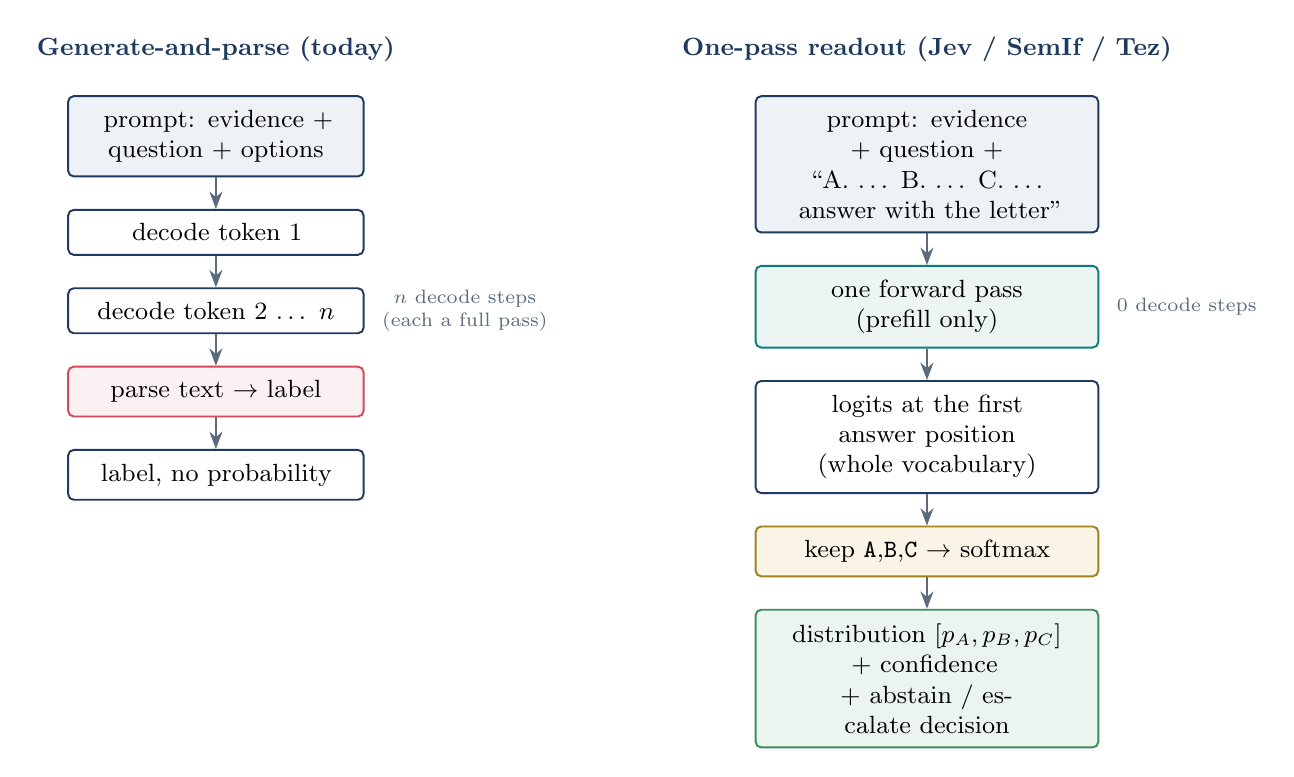
\begin{tikzpicture}[node distance=4mm]
% left: generate
\node[head] (hl) {Generate-and-parse (today)};
\node[boxk,below=3mm of hl,text width=34mm] (p1) {prompt: evidence + question + options};
\node[box,below=of p1,text width=34mm] (d1) {decode token 1};
\node[box,below=of d1,text width=34mm] (d2) {decode token 2 \ldots\ $n$};
\node[boxc,below=of d2,text width=34mm] (pa) {parse text $\to$ label};
\node[box,below=of pa,text width=34mm] (o1) {label, no probability};
\draw[arr] (p1)--(d1); \draw[arr] (d1)--(d2); \draw[arr] (d2)--(pa); \draw[arr] (pa)--(o1);
\node[lbl,right=1mm of d2] {$n$ decode steps\\ (each a full pass)};
% right: one pass
\node[head,right=34mm of hl] (hr) {One-pass readout (Jev / SemIf / Tez)};
\node[boxk,below=3mm of hr,text width=40mm] (p2) {prompt: evidence + question +\\ ``A. \ldots\ B. \ldots\ C. \ldots\ answer with the letter''};
\node[boxt,below=of p2,text width=40mm] (f2) {one forward pass (prefill only)};
\node[box,below=of f2,text width=40mm] (l2) {logits at the first answer position\\ (whole vocabulary)};
\node[boxg,below=of l2,text width=40mm] (m2) {keep \code{A},\code{B},\code{C} $\to$ softmax};
\node[boxl,below=of m2,text width=40mm] (o2) {distribution $[p_A,p_B,p_C]$ + confidence\\ + abstain / escalate decision};
\draw[arr] (p2)--(f2); \draw[arr] (f2)--(l2); \draw[arr] (l2)--(m2); \draw[arr] (m2)--(o2);
\node[lbl,right=1mm of f2] {0 decode steps};
\end{tikzpicture}
\caption{The mechanism. Generation pays $n$ decode steps and returns a label; the one-pass readout pays one prefill and returns a distribution over the declared options. Nothing is sampled or parsed.}
\label{fig:mechanism}
\end{figure}

\subsection{Jev versus a local build}
\begin{figure}[H]
\centering
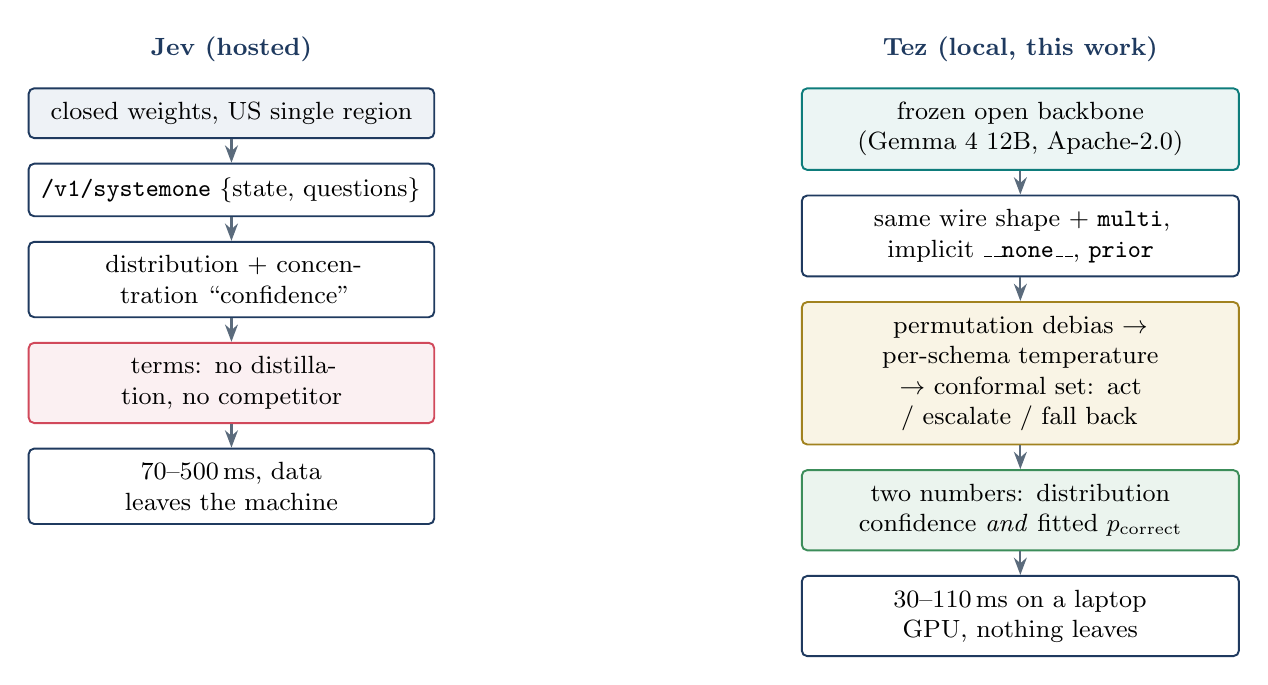
\begin{tikzpicture}[node distance=3mm]
\node[head] (a) {Jev (hosted)};
\node[boxk,below=2mm of a,text width=48mm] (a1) {closed weights, US single region};
\node[box,below=of a1,text width=48mm] (a2) {\code{/v1/systemone} \{state, questions\}};
\node[box,below=of a2,text width=48mm] (a3) {distribution + concentration ``confidence''};
\node[boxc,below=of a3,text width=48mm] (a4) {terms: no distillation, no competitor};
\node[box,below=of a4,text width=48mm] (a5) {70--500\,ms, data leaves the machine};
\draw[arr](a1)--(a2);\draw[arr](a2)--(a3);\draw[arr](a3)--(a4);\draw[arr](a4)--(a5);
\node[head,right=70mm of a] (b) {Tez (local, this work)};
\node[boxt,below=2mm of b,text width=52mm] (b1) {frozen open backbone (Gemma 4 12B, Apache-2.0)};
\node[box,below=of b1,text width=52mm] (b2) {same wire shape + \code{multi}, implicit \code{\_\_none\_\_}, \code{prior}};
\node[boxg,below=of b2,text width=52mm] (b3) {permutation debias $\to$ per-schema temperature\\ $\to$ conformal set: act / escalate / fall back};
\node[boxl,below=of b3,text width=52mm] (b4) {two numbers: distribution confidence \emph{and} fitted $p_\text{correct}$};
\node[box,below=of b4,text width=52mm] (b5) {30--110\,ms on a laptop GPU, nothing leaves};
\draw[arr](b1)--(b2);\draw[arr](b2)--(b3);\draw[arr](b3)--(b4);\draw[arr](b4)--(b5);
\end{tikzpicture}
\caption{Jev as documented versus the local stack built here. The technique is shared; the differences are openness, the calibration contract, and where the data lives.}
\end{figure}

% ================================================================ 3
\section{How the technique works, and what the literature predicts}
\label{sec:method}

\subsection{The readout, precisely}
Let $x$ be the rendered prompt (chat template, evidence, question, options with letters $\ell_1\ldots\ell_k$, an instruction to answer with the letter, and the generation prompt). One forward pass yields logits $z\in\mathbb{R}^{|V|}$ at the first answer position. With $t(\ell_i)$ the token id of letter $\ell_i$, the option distribution is
\[
p_i \;=\; \frac{\exp z_{t(\ell_i)}}{\sum_{j=1}^{k}\exp z_{t(\ell_j)}} .
\]
Two invariants make the read position unambiguous, both enforced by the harness: every letter must be a single round-trip token, and \code{prompt + letter} must tokenise to \code{prompt} followed by exactly that token (no merge across the boundary). Because a server's returned log-probabilities are already log-softmax over $V$, restricting and renormalising them equals the softmax over raw slot logits.

\subsection{Why it works at all: symbol binding}
The method assumes the model can \emph{bind} the semantics of an option to its letter. Robinson and Wingate \cite{mcsb} showed this multiple-choice symbol binding is an emergent, scale-gated ability; Wong, Nouwen and Gatt \cite{twostage} showed it is computed in two stages --- the winner is decided in content space, then bound to a symbol later in the network. The readout only taps stage two (Fig.~\ref{fig:twostage}). A small model may know the answer and still fail to route it to the letter; that failure looks like order sensitivity, and it is exactly what our 3B and 4B results show (\S\ref{sec:scale}).

\begin{figure}[H]
\centering
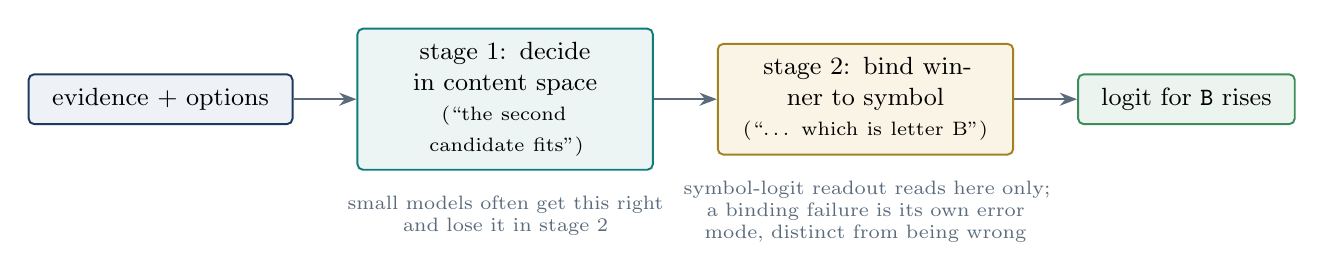
\begin{tikzpicture}[node distance=5mm]
\node[boxk,text width=30mm] (in) {evidence + options};
\node[boxt,right=8mm of in,text width=34mm] (s1) {stage 1: decide in content space\\ \scriptsize (``the second candidate fits'')};
\node[boxg,right=8mm of s1,text width=34mm] (s2) {stage 2: bind winner to symbol\\ \scriptsize (``\ldots\ which is letter B'')};
\node[boxl,right=8mm of s2,text width=24mm] (out) {logit for \code{B} rises};
\draw[arr](in)--(s1);\draw[arr](s1)--(s2);\draw[arr](s2)--(out);
\node[lbl,below=2mm of s2,text width=50mm] {symbol-logit readout reads here only; a binding failure is its own error mode, distinct from being wrong};
\node[lbl,below=2mm of s1,text width=40mm] {small models often get this right\\ and lose it in stage 2};
\end{tikzpicture}
\caption{The two-stage account of multiple-choice answering \cite{twostage} and where the readout taps it.}
\label{fig:twostage}
\end{figure}

\subsection{What each paper changes in the build}
\begin{table}[H]
\centering\small
\begin{tabularx}{\textwidth}{L{38mm} X L{48mm}}
\toprule
Paper & Finding & Consequence here \\
\midrule
PET \cite{pet}; LM-BFF \cite{lmbff} & meaningful label words beat bare symbols; label-word choice swings accuracy & \code{A/B/C} is the weakest verbalizer; an ablation to run \\
Surface-form competition \cite{sfc} & scoring option \emph{text} splits mass across synonyms & symbol scoring sidesteps this --- an argument \emph{for} the design \\
Calibrate before use \cite{zhao} & content-free input exposes label bias; divide it out & \hl{harmful here} (\S\ref{sec:calib}); never with an abstain option \\
MCSB \cite{mcsb}; two-stage \cite{twostage} & binding is scale-gated and late & screen the backbone by measuring it \\
PriDe \cite{pride} & selection bias is mostly token bias on option IDs & measured: flat prior on Gemma 4, so a no-op there \\
Position bias vs.\ option count \cite{leeson} & bias grows with more options & stress-test above production $N$ \\
Mind the gap \cite{gap} & bare vs space-prefixed letters differ & read the token the template produces \\
\bottomrule
\end{tabularx}
\caption{The reading list and what it changed.}
\end{table}

\subsection{What ``calibrated'' has to mean}
The distribution above is a \emph{conditional option score}; it is not $P(\text{correct})$ until it is made so. The contract adopted here: temperature scaling per schema, fitted out-of-fold with folds split by source group; \emph{conformal} sets mapped onto orchestration (set size 1 $\to$ act; $>1$ $\to$ escalate; empty $\to$ fall back to the full LLM), Mondrian so rare costly classes get their own quantile; log-loss and Brier as primary metrics, binned ECE secondary; risk--coverage and AURC for abstention. Post-hoc calibration is sufficient for v1: the AWS decision-token study \cite{awsdt} shows isotonic regression closes most of the gap that calibration-aware RL claims.

% ================================================================ 4
\section{Experimental setup}
\label{sec:setup}

\textbf{Hardware.} NVIDIA RTX 5080 Laptop GPU (16\,GB), Intel Core Ultra 9 275HX (no AVX-512), Windows 11.\quad
\textbf{Engines.} (a) llama.cpp b11100 \code{win-cuda-13.4}, \code{llama-server}, full offload, one slot, fresh scoring (\code{cache\_prompt=false}) for every accuracy and calibration run; (b) \code{transformers} 5.8 / torch 2.10 in-process, BF16, \code{logits\_to\_keep=1}, CUDA-synchronised timing.\quad
\textbf{Models.} Gemma 4 12B (Q8\_0 and Q4\_K\_M; Apache-2.0; thinking disabled), Gemma 3 4B Q4\_K\_M (fresh ggml-org GGUF), Llama 3.2 3B Q4\_K\_M, Qwen3.5-4B and Qwen3-4B BF16. Every server run asserts the loaded model path from \code{/props}.\quad
\textbf{Prompt.} Byte-identical to SemIf's \code{direct-options-v1}, built by importing SemIf's own \code{core.py}, rendered into each model's chat template with the generation prompt appended; for Gemma 4 the empty thought channel \code{<|channel>thought\textbackslash n<channel|>} is included and the letter is read at the next position.\quad
\textbf{Readout.} \code{n\_predict=1, temperature=0, n\_probs=200}; top-1 token and any missing letter logged (none missing on benchmark rows; top-1 always a declared letter).\quad
\textbf{Data.} SemIf's frozen fixtures: \code{authored144} (three families $\times$ 48 rows, three options each) and \code{perturbations108} (36 originals $\times$ option reversal / criterion re-wrap / irrelevant context). Labels are model-reviewed, not human-adjudicated; the data are public, so this is a reproduction, not a held-out claim. Gemma 4 12B (June 2026) predates the fixtures (September 2026).\quad
\textbf{Metrics.} Mean-family balanced accuracy with classes keyed by \emph{option id}, source-group bootstrap 95\% CI; NLL and Brier; ECE-15; option-id-matched flip rate with Wilson CI and total-variation distance for perturbations; AUROC of max-probability as error detector; AURC; exact McNemar for paired model comparisons.\quad
\textbf{Determinism.} Three independent Q8\_0 runs were byte-identical in every probability.

% ================================================================ 5
\section{Results on the SemIf benchmark}
\label{sec:experiments}

\subsection{Headline and scale}
\label{sec:scale}

\begin{table}[H]
\centering\small
\resizebox{\textwidth}{!}{%
\begin{tabular}{l r r r r r r}
\toprule
Model (frozen) & Authored mfba (95\% CI) & Perturb. & NLL raw$\to$best & Brier raw$\to$best & Reversal flips/36 & p50 \\
\midrule
\textbf{Gemma 4 12B Q8\_0} & \textbf{0.943} (0.897--0.981) & \textbf{0.992} & 0.478$\to$\textbf{0.158} & 0.094$\to$\textbf{0.075} & \textbf{0} ($\le$9.6\%) & 110\,ms \\
Gemma 4 12B Q4\_K\_M & 0.918 (0.871--0.958) & 0.981 & 0.549$\to$0.184 & 0.130$\to$0.092 & 1 & 100\,ms \\
Qwen3.5-4B BF16 (in-process) & 0.813 (0.755--0.865) & --- & 0.427 & 0.248 & --- & 224\,ms$^\dagger$ \\
\quad + 6-permutation average & \textbf{0.912} & --- & --- & --- & --- & 321\,ms$^\dagger$ \\
Qwen3-4B BF16 (in-process) & 0.740 (0.676--0.809) & --- & --- & --- & --- & 75\,ms$^\dagger$ \\
\quad + 6-permutation average & 0.832 & --- & --- & --- & --- & 204\,ms$^\dagger$ \\
Gemma 3 4B Q4\_K\_M & 0.646 (0.570--0.728) & 0.729 & 3.433$\to$0.696 & 0.661$\to$0.397 & 13 (36\%) & 40\,ms \\
Llama 3.2 3B Q4\_K\_M & 0.358 (0.319--0.399) & 0.496 & 1.673$\to$1.043 & 0.827$\to$0.627 & 10 (28\%) & 25\,ms \\
\emph{SemIf published: 4B / 27B} & \emph{0.813 / 0.958} & \emph{0.766 / ---} & & & & \\
\bottomrule
\end{tabular}}
\caption{Decision quality on SemIf's \code{authored144} and \code{perturbations108}. ``best'' = six-permutation average + out-of-fold temperature. $^\dagger$transformers timing, not comparable with llama.cpp.}
\label{tab:main}
\end{table}

\begin{figure}[H]
\centering
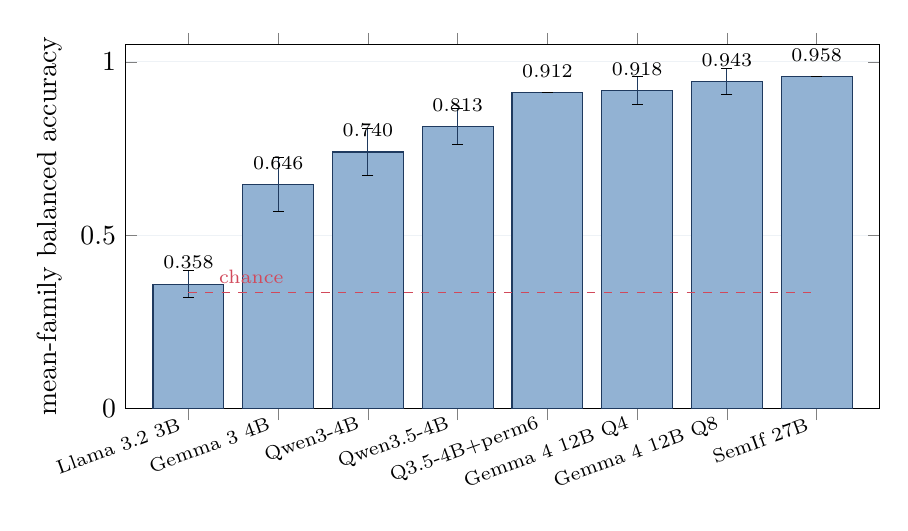
\begin{tikzpicture}
\begin{axis}[width=0.92\textwidth,height=62mm,ybar,bar width=9mm,ymin=0,ymax=1.05,
  ylabel={mean-family balanced accuracy},xtick=data,
  symbolic x coords={Llama 3.2 3B,Gemma 3 4B,Qwen3-4B,Qwen3.5-4B,Q3.5-4B+perm6,Gemma 4 12B Q4,Gemma 4 12B Q8,SemIf 27B},
  x tick label style={rotate=20,anchor=east,font=\scriptsize},ymajorgrids,grid style={mist},
  error bars/y dir=both,error bars/y explicit,nodes near coords,every node near coord/.append style={font=\scriptsize,yshift=2pt},
  point meta=explicit symbolic]
\addplot[fill=sky!60,draw=navy] coordinates {
 (Llama 3.2 3B,0.358) +- (0.039,0.039) [0.358]
 (Gemma 3 4B,0.646) +- (0.076,0.079) [0.646]
 (Qwen3-4B,0.740) +- (0.064,0.069) [0.740]
 (Qwen3.5-4B,0.813) +- (0.058,0.052) [0.813]
 (Q3.5-4B+perm6,0.912) +- (0,0) [0.912]
 (Gemma 4 12B Q4,0.918) +- (0.047,0.040) [0.918]
 (Gemma 4 12B Q8,0.943) +- (0.046,0.038) [0.943]
 (SemIf 27B,0.958) +- (0,0) [0.958]};
\draw[dashed,coral] (axis cs:Llama 3.2 3B,0.333) -- (axis cs:SemIf 27B,0.333) node[pos=0.1,above,font=\scriptsize,color=coral] {chance};
\end{axis}
\end{tikzpicture}
\caption{The scale curve on one dataset and one prompt (95\% bootstrap CIs where available). Permutation averaging moves the 4B most of the way to the 12B.}
\label{fig:scale}
\end{figure}

\paragraph{Paired significance (exact McNemar, same 144 rows).} 12B Q8 vs Qwen3.5-4B: 24 rows only the 12B gets right vs 3 only the 4B, $p=5\times10^{-5}$. 12B Q8 vs Gemma 3 4B: 44 vs 3, $p=2\times10^{-10}$. 12B Q8 vs Q4: 3 vs 0, $p=0.25$ (not significant). Qwen3.5-4B six-permutation vs fresh: 18 fixed, 2 broken, $p=4\times10^{-4}$. \hl{12B Q8 vs Qwen3.5-4B + permutations: 7 vs 2, $p=0.18$.} SemIf's published 0.813 reproduced exactly (0.8132) through \code{apply\_chat\_template(enable\_thinking=False)}, anchoring every other number to a published baseline.

\paragraph{Reading.} A frozen 12B is clearly above the published 4B but is mid-scale (SemIf's 27B: 0.958). Sub-4B decoders are at or near chance with high order sensitivity, and no post-hoc method moves them --- calibration cannot create knowledge. The 4B models sit in between and gain 7--10 points from permutation averaging: they \emph{have} the knowledge and lose it in binding, which is exactly the two-stage prediction.

\subsection{Perturbations and order bias}
\begin{table}[H]
\centering\small
\begin{tabular}{l r r r r}
\toprule
Gemma 4 12B Q8\_0, 36 pairs each & flips & flip rate (Wilson 95\%) & TV distance & acc.\ base$\to$pert. \\
\midrule
option\_reversal & 0 & 0\% (0--9.6\%) & 0.002 & 1.000$\to$1.000 \\
criterion\_wrapper & 1 & 2.8\% (0.5--14\%) & 0.025 & 1.000$\to$0.972 \\
irrelevant\_context & 0 & 0\% (0--9.6\%) & 0.006 & 1.000$\to$1.000 \\
\midrule
\multicolumn{5}{p{140mm}}{All six orderings scored: letter mass A/B/C = 0.331/0.336/0.333; all six orderings agree on the argmax for 95.8\% of rows; PriDe prior correction is a no-op} \\
\bottomrule
\end{tabular}
\caption{Stability under SemIf's perturbations and the full-permutation order-bias measurement. ``0/36'' bounds the true flip rate at $\le$9.6\%, not at zero.}
\end{table}

\subsection{Calibration and debiasing}
\label{sec:calib}
\begin{table}[H]
\centering\small
\begin{tabular}{l r r r r r r}
\toprule
Method (Q8\_0, 144 rows, OOF temperature by group) & Acc & NLL & Brier & ECE-15 & AUROC(err) & AURC \\
\midrule
raw & 0.951 & 0.478 & 0.094 & 0.047 & 0.834 & 0.013 \\
temperature (OOF) & 0.951 & 0.193 & 0.083 & 0.027 & 0.807 & 0.016 \\
2-permutation average & 0.958 & 0.393 & 0.089 & 0.047 & 0.873 & 0.007 \\
6-permutation average & 0.951 & 0.281 & 0.083 & 0.038 & \textbf{0.933} & \textbf{0.005} \\
\textbf{6-permutation + temperature} & 0.951 & \textbf{0.158} & \textbf{0.075} & 0.037 & 0.906 & 0.006 \\
contextual calibration, ``N/A'' \cite{zhao} & \hl{0.778} & 1.707 & 0.355 & 0.162 & 0.928 & 0.047 \\
contextual, 3-placeholder average & 0.847 & 1.299 & 0.272 & 0.121 & 0.861 & 0.036 \\
\quad damped $\alpha=0.25$ & 0.951 & 0.564 & 0.092 & 0.046 & 0.800 & 0.014 \\
\bottomrule
\end{tabular}
\caption{Post-hoc calibration and debiasing. Accuracy is plain accuracy. Six orderings beat two on every proper score and give the best error detection: disagreement between orderings is the best uncertainty signal the frozen model has.}
\label{tab:calib}
\end{table}

\begin{figure}[H]
\centering
\begin{subfigure}{0.48\textwidth}
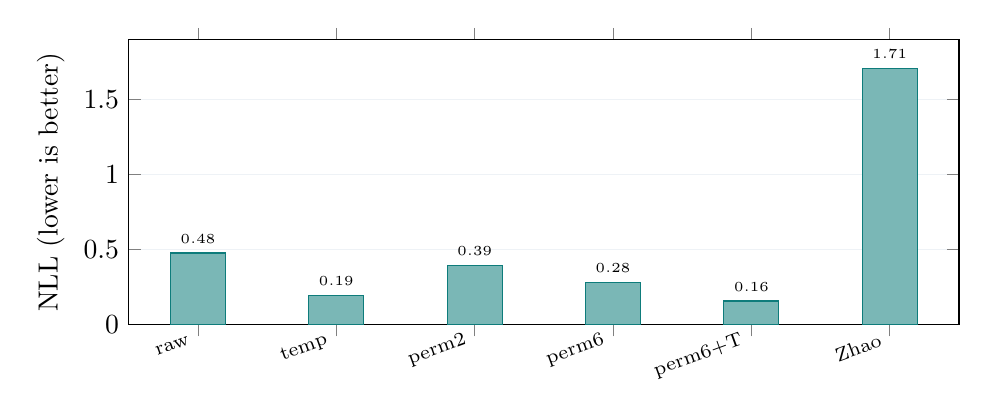
\begin{tikzpicture}
\begin{axis}[width=\textwidth,height=52mm,ybar,bar width=7mm,ymin=0,ymax=1.9,ylabel={NLL (lower is better)},xtick=data,
 symbolic x coords={raw,temp,perm2,perm6,perm6+T,Zhao},x tick label style={font=\scriptsize,rotate=20,anchor=east},ymajorgrids,grid style={mist},
 nodes near coords,every node near coord/.append style={font=\tiny}]
\addplot[fill=teal!55,draw=teal] coordinates {(raw,0.478)(temp,0.193)(perm2,0.393)(perm6,0.281)(perm6+T,0.158)(Zhao,1.707)};
\end{axis}
\end{tikzpicture}
\caption{Negative log-likelihood.}
\end{subfigure}\hfill
\begin{subfigure}{0.48\textwidth}
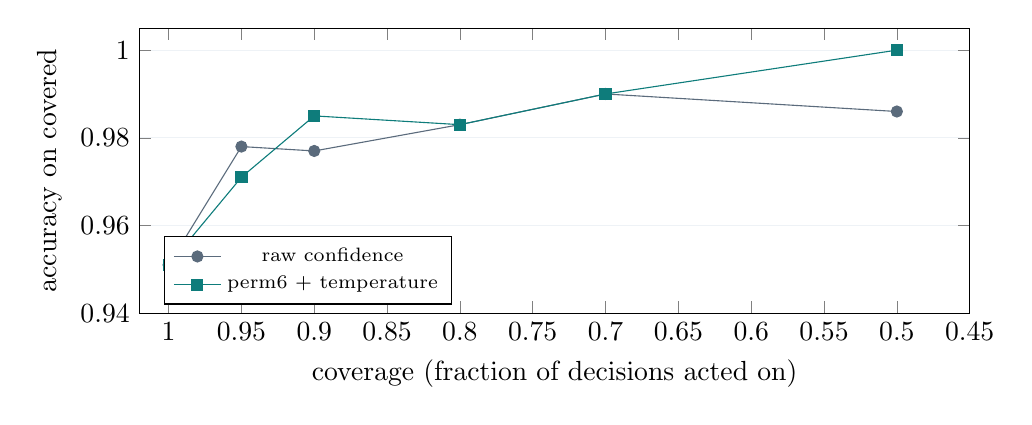
\begin{tikzpicture}
\begin{axis}[width=\textwidth,height=52mm,xlabel={coverage (fraction of decisions acted on)},ylabel={accuracy on covered},
 xmin=0.45,xmax=1.02,ymin=0.94,ymax=1.005,ymajorgrids,grid style={mist},legend pos=south west,legend style={font=\scriptsize},x dir=reverse]
\addplot[color=slate,mark=*] coordinates {(1.0,0.951)(0.95,0.978)(0.9,0.977)(0.8,0.983)(0.7,0.990)(0.5,0.986)};
\addplot[color=teal,mark=square*] coordinates {(1.0,0.951)(0.95,0.971)(0.9,0.985)(0.8,0.983)(0.7,0.990)(0.5,1.000)};
\legend{raw confidence,perm6 + temperature}
\end{axis}
\end{tikzpicture}
\caption{Risk--coverage: abstain on the least confident.}
\end{subfigure}
\caption{Calibration recipes. Abstaining on the least-confident 10\% lifts accuracy to $\approx$0.98; the residual errors are confidently wrong ``should have said insufficient'' rows.}
\end{figure}

\paragraph{Why contextual calibration fails here.} With the evidence replaced by ``N/A'', ``[MASK]'' or the empty string, Gemma 4 chose \emph{insufficient} in 144/144/143 rows at mean max-probability 0.999. That is the \emph{correct} answer to an evidence-free question, not a label bias; dividing by it deletes the 36 rows whose gold answer genuinely is \emph{insufficient}. Rule: never apply content-free correction when the option set contains an ``insufficient / unknown / none'' answer that empty input should legitimately select --- which, for a decision model built around abstention, is most option sets.

\paragraph{Error analysis.} 7 misses in 144 at Q8; six have gold = \emph{insufficient}, all at $p>0.97$: over-commitment, the classic instruct-model failure, and precisely what an abstention layer exists to catch. Six-permutation disagreement flags it better than raw confidence (AUROC 0.933 vs 0.834).

% ================================================================ 6
\section{Systems: prompt layout and the cache decide latency}
\label{sec:systems}

The first draft of this work concluded that llama-server had a ``$\sim$110\,ms fixed floor'' and ``no partial-prefix reuse''. Both were an artefact of one flag. Gemma 3/4 use sliding-window attention on most layers; llama.cpp's SWA cache cannot be rolled back to an earlier position, so when a request shares a prefix with the cached one the server silently re-evaluates the whole prompt (\code{timings.prompt\_n} never drops). \code{--swa-full} allocates a full cache for those layers and prefix reuse works as documented. The second lever is the prompt itself: whatever is \emph{constant across the decisions about to be made} must come first (Fig.~\ref{fig:layout}).

\begin{figure}[H]
\centering
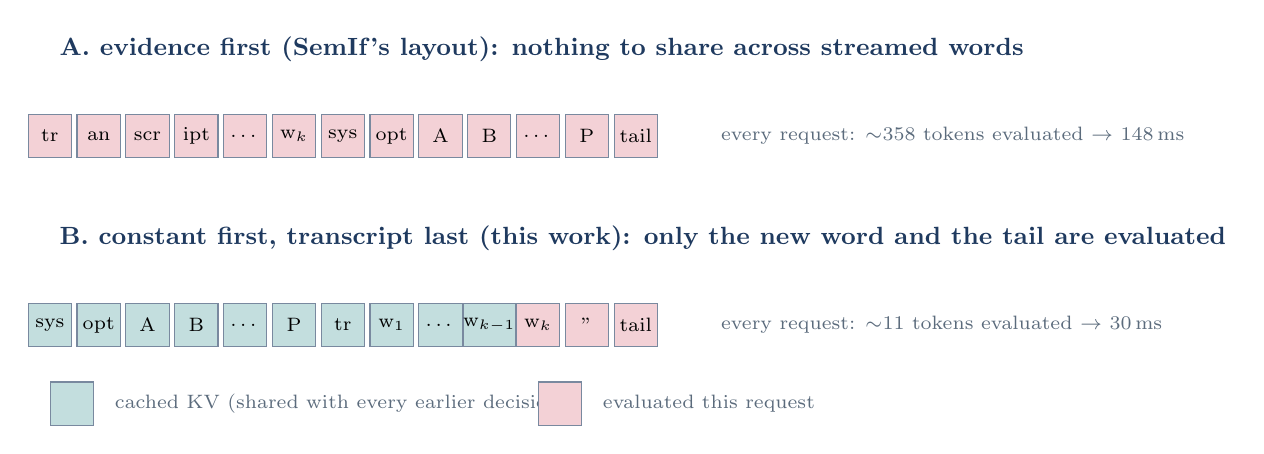
\begin{tikzpicture}[node distance=1.2mm]
\node[head,anchor=west] at (0,1.1) {A. evidence first (SemIf's layout): nothing to share across streamed words};
\foreach \i/\s/\t in {0/toke/tr,1/toke/an,2/toke/scr,3/toke/ipt,4/toke/\ldots,5/toke/w$_k$,6/toke/sys,7/toke/opt,8/toke/A,9/toke/B,10/toke/\ldots,11/toke/P,12/toke/tail}
  \node[\s] (a\i) at (\i*0.62,0) {\t};
\node[lbl,anchor=west] at (8.4,0) {every request: $\sim$358 tokens evaluated $\to$ 148\,ms};
\node[head,anchor=west] at (0,-1.3) {B. constant first, transcript last (this work): only the new word and the tail are evaluated};
\foreach \i/\s/\t in {0/tokc/sys,1/tokc/opt,2/tokc/A,3/tokc/B,4/tokc/\ldots,5/tokc/P,6/tokc/tr,7/tokc/w$_1$,8/tokc/\ldots,9/tokc/w$_{k-1}$,10/toke/w$_k$,11/toke/",12/toke/tail}
  \node[\s] (b\i) at (\i*0.62,-2.4) {\t};
\node[lbl,anchor=west] at (8.4,-2.4) {every request: $\sim$11 tokens evaluated $\to$ 30\,ms};
\node[tokc,anchor=west] at (0,-3.4) {}; \node[lbl,anchor=west] at (0.7,-3.4) {cached KV (shared with every earlier decision)};
\node[toke,anchor=west] at (6.2,-3.4) {}; \node[lbl,anchor=west] at (6.9,-3.4) {evaluated this request};
\end{tikzpicture}
\caption{Prompt layout as a systems decision. The token count and timings are measured on the Gemma 4 12B Q8\_0 voice prompt (\S\ref{sec:voice}); with the SWA cache defaulted, layout B still evaluated all 394 tokens.}
\label{fig:layout}
\end{figure}

\begin{table}[H]
\centering\small
\resizebox{\textwidth}{!}{%
\begin{tabular}{l r r r}
\toprule
Gemma 4 12B Q8\_0, voice prompt & tokens evaluated & prompt\_ms p50/p95 & HTTP round-trip p50/p95 \\
\midrule
default server, each streamed word & 394--397 (all) & 205 / --- & 230 / --- \\
\code{--swa-full}, each streamed word & \textbf{11} & \textbf{30 / 36} & \textbf{45 / 56} \\
\code{--swa-full}, first word of a new utterance & 11 & 31 & 45 \\
\code{--swa-full}, after an action fired (33-token \code{prior} line) & 33 & $\sim$55 & $\sim$70 \\
\code{n\_probs} 32 instead of 200 (letters fall off the list) & 11 & 32 & 49 (no gain) \\
transcript first (SemIf order), cached & 358 & 148 / 179 & 221 / 252 \\
fresh 142-token benchmark rows & 142 & 110 / 122 & 178 / 203 \\
\midrule
Qwen3-4B in-process: fresh / prefix reuse / 6-perm batch & 148 / 83 / 6$\times$148 & 75 / 54 / 204 & --- \\
\bottomrule
\end{tabular}}
\caption{Latency. Per-decision cost is proportional to the uncached suffix ($\approx$2.7\,ms per token on the 12B Q8 here) plus $\approx$15\,ms of HTTP/JSON, removable in-process. Cached vs fresh in-process differed in argmax on 2/144 rows (TV 0.008) --- SemIf's documented regime.}
\label{tab:latency}
\end{table}

\begin{figure}[H]
\centering
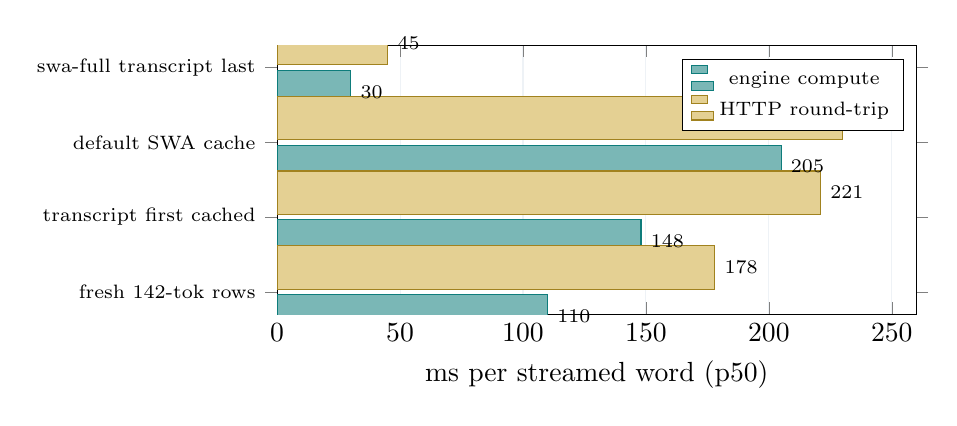
\begin{tikzpicture}
\begin{axis}[width=0.8\textwidth,height=50mm,xbar,bar width=5.5mm,xmin=0,xmax=260,xlabel={ms per streamed word (p50)},ytick=data,
 symbolic y coords={fresh 142-tok rows,transcript first cached,default SWA cache,swa-full transcript last},y tick label style={font=\scriptsize},
 xmajorgrids,grid style={mist},nodes near coords,every node near coord/.append style={font=\scriptsize},legend style={font=\scriptsize,at={(0.98,0.95)},anchor=north east}]
\addplot[fill=teal!55,draw=teal] coordinates {(30,swa-full transcript last)(205,default SWA cache)(148,transcript first cached)(110,fresh 142-tok rows)};
\addplot[fill=gold!50,draw=gold!80!black] coordinates {(45,swa-full transcript last)(230,default SWA cache)(221,transcript first cached)(178,fresh 142-tok rows)};
\legend{engine compute,HTTP round-trip}
\end{axis}
\end{tikzpicture}
\caption{Same model, same readout: the 7$\times$ comes from layout and cache configuration, not from a smaller model.}
\end{figure}

\paragraph{The crossover rule.} An encoder cannot cache context (every option changes the whole representation) and pays full context per decision; a decoder caches the constant part and scores short suffixes. One context $\to$ many decisions favours the cached decoder ($\sim$5$\times$); one $\to$ one favours the encoder ($\sim$10$\times$). The voice case is the degenerate version: the option list is the constant and each new word is the suffix.

\paragraph{Precision.} Q4\_K\_M$\to$Q8\_0 moved probability mass on $\sim$3\% of decisions; every argmax that moved was a Q4 error being corrected, for $\sim$10\,ms. Weights at Q8 are the floor for calibration work; the KV cache and \code{lm\_head} stay unquantised; any change to quantisation or caching is a new model and must be re-measured against a fresh reference.

% ================================================================ 7
\section{Where it applies}
\label{sec:apps}

\begin{figure}[H]
\centering
\begin{tikzpicture}
\node[boxt,text width=34mm,minimum height=16mm] (hub) at (0,0) {\textbf{one pass}\\ state + typed question\\ $\to$ distribution + confidence};
\node[box,text width=30mm] (a1) at (-5.6,2.4) {agent loop control\\ \scriptsize continue / review / stop};
\node[box,text width=30mm] (a2) at (0,3.0) {tool / agent / model routing\\ \scriptsize shortlist top 3--7, escalate on doubt};
\node[box,text width=30mm] (a3) at (5.6,2.4) {risky-action gate\\ \scriptsize asymmetric: block on low $P$(safe)};
\node[box,text width=30mm] (a4) at (-6.2,0) {triage / classification\\ \scriptsize email, tickets, documents};
\node[box,text width=30mm] (a5) at (6.2,0) {RAG relevance / guardrails\\ \scriptsize one state, many yes/no};
\node[boxg,text width=30mm] (a6) at (-5.6,-2.4) {\textbf{voice $\to$ action}\\ \scriptsize streamed, early commit (\S\ref{sec:voice})};
\node[box,text width=30mm] (a7) at (0,-3.0) {computer use\\ \scriptsize one scored pass replaces reasoning + action emission};
\node[box,text width=30mm] (a8) at (5.6,-2.4) {evidence-supports-X / judge\\ \scriptsize NLI-style, flip rate matters};
\foreach \n in {a1,a2,a3,a4,a5,a6,a7,a8} \draw[arr] (hub)--(\n);
\end{tikzpicture}
\caption{Decision types that fit the primitive. The one architectural finding shared by all of them: decomposition wins (a third-party audit of Jev: 62.6\% on ``is this phishing?'' versus 95\% on five narrow sub-questions plus a rule), so the primitive is one state $\to$ many independent typed questions --- the shape that needs prefix reuse.}
\end{figure}

\paragraph{Computer use, honestly.} Action spaces are tiny (OS-Atlas collapses 17 types to 10) and scoring a fixed action set is established (SayCan; ActionRank: 247 vs 632\,ms, $-2.6$ points, 0\% invalid). But per-step time on OSWorld-Human is planning 53--75\%, reflection 22--34\%, grounding and execution 2--4\%: the action \emph{name} is single-digit percent of the tokens, so replacing it alone attacks noise. The version that works replaces the whole reasoning-plus-action emission with one scored pass, gated by confidence, falling back to full reasoning on doubt, paired with attention-based grounding so coordinates need no tokens either. The voice loop below is the text-only special case of that design, and its commit policy transfers directly.

\paragraph{What a small model can be trusted with.} Routers plateau at 60--75\% regardless of architecture and guardrail classifiers top out around F1 0.73--0.76. Trust: shortlisting, cheap-vs-expensive routing with escalate-on-doubt, recall-first pre-filters, cheap reversible actions on a calibrated early signal. Never: auto-approving irreversible actions, or escalation calls on novel cases --- the model may raise scrutiny, never lower it.

% ================================================================ 8
\section{Case study: voice command $\to$ instant action}
\label{sec:voice}

\subsection{Task and data}
Sixteen actions (\code{open\_notes}, \code{type\_text}, \code{open\_youtube}, \code{play\_youtube}, \code{open\_spotify}, \code{play\_liked\_songs}, \code{play\_spotify}, \code{pause}/\code{resume}/\code{next}, \code{volume\_up}/\code{down}, \code{open\_browser}, \code{search\_web}, \code{close\_app}, \code{none}) and 220 labelled utterances in six styles: canonical (77), paraphrase (55), noisy with fillers and ASR-like errors (33), compound ``open X and do Y'' (22; first action as \code{intent}, second as \code{then}), ambiguous (11; accepted \code{alt}) and out-of-scope (22). Each row carries a human-annotated \emph{commit word}: the earliest word at which a listener knows the action. All 220 were synthesised to 16\,kHz WAV with Windows SAPI so the ASR stage could be timed on audio.

\begin{figure}[H]
\centering
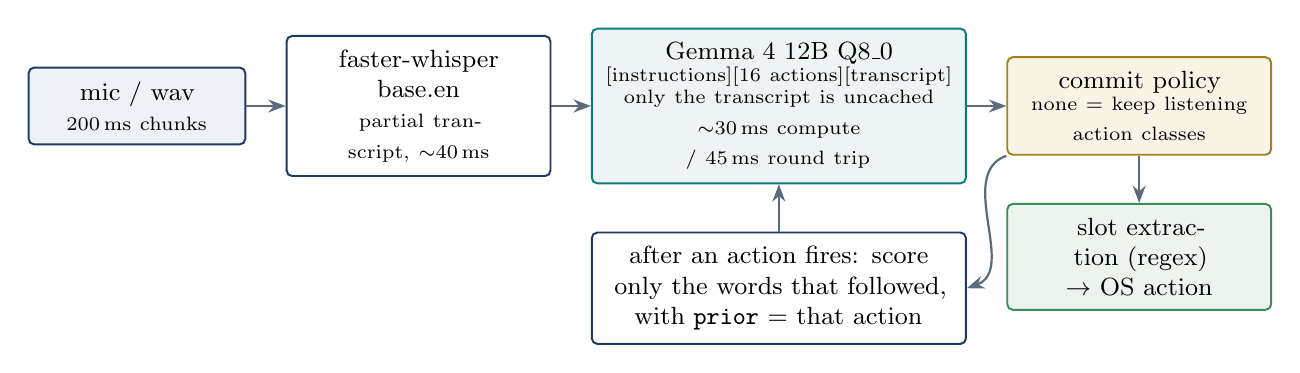
\begin{tikzpicture}[node distance=5mm]
\node[boxk,text width=24mm] (mic) {mic / wav\\ \scriptsize 200\,ms chunks};
\node[box,right=of mic,text width=30mm] (asr) {faster-whisper base.en\\ \scriptsize partial transcript, $\sim$40\,ms};
\node[boxt,right=of asr,text width=44mm] (dec) {Gemma 4 12B Q8\_0\\ \scriptsize [instructions][16 actions][transcript]\\ only the transcript is uncached\\ $\sim$30\,ms compute / 45\,ms round trip};
\node[boxg,right=of dec,text width=30mm] (pol) {commit policy\\ \scriptsize none = keep listening\\ action classes};
\node[boxl,below=6mm of pol,text width=30mm] (act) {slot extraction (regex)\\ $\to$ OS action};
\node[box,below=6mm of dec,text width=44mm] (res) {after an action fires: score only the words that followed, with \code{prior} = that action};
\draw[arr](mic)--(asr);\draw[arr](asr)--(dec);\draw[arr](dec)--(pol);\draw[arr](pol)--(act);
\draw[arr](pol.south west) to[out=200,in=20] (res.east);
\draw[arr](res.north) -- (dec.south);
\end{tikzpicture}
\caption{The pipeline. Every partial transcript is one typed decision; the model never generates.}
\end{figure}

\subsection{Decision quality on the full utterance}
\begin{table}[H]
\centering\small
\begin{tabular}{l r r r}
\toprule
Gemma 4 12B Q8\_0, 220 utterances & transcript last (used) & transcript first (control) & ``still speaking'' wording \\
\midrule
Intent accuracy, strict & \textbf{0.905} & 0.877 & 0.868 \\
Accepting \code{then} / \code{alt} labels & \textbf{0.982} & 0.955 & 0.968 \\
canonical / paraphrase / noisy & 1.000 / 0.964 / 0.970 & 1.000 / 0.945 / 0.909 & 1.000 / 0.982 / 0.939 \\
compound (strict; routes to the \emph{last} verb) & 0.273 & 0.318 & 0.045 \\
ambiguous & 0.818 & 0.636 & 0.727 \\
out-of-scope $\to$ \code{none}: recall / precision & 1.000 / \textbf{0.917} & 0.909 / 0.769 & 0.909 / 0.833 \\
per-word cost (compute / round trip) & \textbf{30 / 45\,ms} & 148 / 221\,ms & 30 / 45\,ms \\
\bottomrule
\end{tabular}
\caption{Moving the transcript after the option list improved accuracy \emph{and} removed 85\% of the latency. Telling the model the transcript may be cut off made it worse everywhere.}
\end{table}

\subsection{Streaming and early commit}
Every word prefix of every utterance was scored (1,158 decisions). After one word the model says \code{none} at $p\approx1$ for 74\% of actionable utterances --- correctly: ``open'' is not yet a command (Fig.~\ref{fig:stream}). A naive ``commit when $p\ge0.9$'' therefore fires \code{none} at word~1 and is 17\% accurate. \hl{The single rule that makes early commit work: a confident \code{none} on a prefix never commits.}

\begin{figure}[H]
\centering
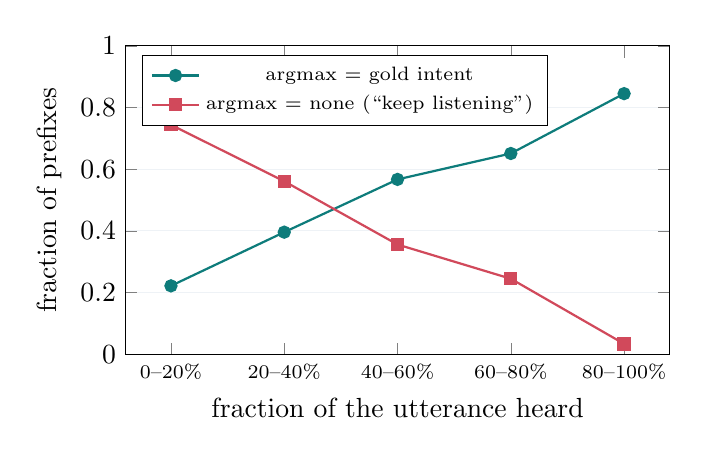
\begin{tikzpicture}
\begin{axis}[width=0.7\textwidth,height=55mm,xlabel={fraction of the utterance heard},ylabel={fraction of prefixes},xtick={0.1,0.3,0.5,0.7,0.9},xticklabels={0--20\%,20--40\%,40--60\%,60--80\%,80--100\%},ymin=0,ymax=1,ymajorgrids,grid style={mist},legend pos=north west,legend style={font=\scriptsize},x tick label style={font=\scriptsize}]
\addplot[color=teal,mark=*,thick] coordinates {(0.1,0.222)(0.3,0.396)(0.5,0.567)(0.7,0.651)(0.9,0.845)};
\addplot[color=coral,mark=square*,thick] coordinates {(0.1,0.744)(0.3,0.561)(0.5,0.356)(0.7,0.245)(0.9,0.034)};
\legend{argmax = gold intent,argmax = none (``keep listening'')}
\end{axis}
\end{tikzpicture}
\caption{What the model says on partial transcripts (198 actionable utterances, transcript-last prompt). Uncertainty is expressed as \code{none}, not as a flat distribution; non-\code{none} predictions at $p\ge0.9$ are 88\% correct on prefixes and 98\% on the earlier SemIf-order run.}
\label{fig:stream}
\end{figure}

\begin{table}[H]
\centering\small
\resizebox{\textwidth}{!}{%
\begin{tabular}{l r r r r}
\toprule
Policy (198 actionable utterances) & commits & acc.\ at commit strict / accepting & mean commit word (of 5.4) & at/before human word \\
\midrule
naive $p\ge0.9$ (any label) & 100\% & 0.172 & 1.0 & 99\% \\
non-none, $p\ge0.9$, stable 1 & 98.5\% & 0.918 / 0.928 & 2.5 & 93\% \\
non-none, $p\ge0.99$, stable 1 & 97.0\% & 0.932 / 0.938 & 2.7 & 89\% \\
non-none, $p\ge0.9$, stable 2 & 76.3\% & 0.960 / 0.967 & 3.5 & 21\% \\
\bottomrule
\end{tabular}}
\caption{Commit policies. The wrong commits at stability 1 are almost all ``youtube \ldots'' $\to$ \code{open\_youtube} before ``play lofi'' arrives: refinable, not wrong, in a live assistant.}
\end{table}

\subsection{Action classes: commit early, refine later}
The right question for a live assistant is not ``was the commit the gold label'' but ``did anything wrong \emph{and costly} happen''. Opening YouTube while the user is still speaking is the point; ``youtube play lofi'' then refines that open into a search rather than contradicting it. Actions are therefore graded by the cost of a wrong early fire (Fig.~\ref{fig:policy}).

\begin{figure}[H]
\centering
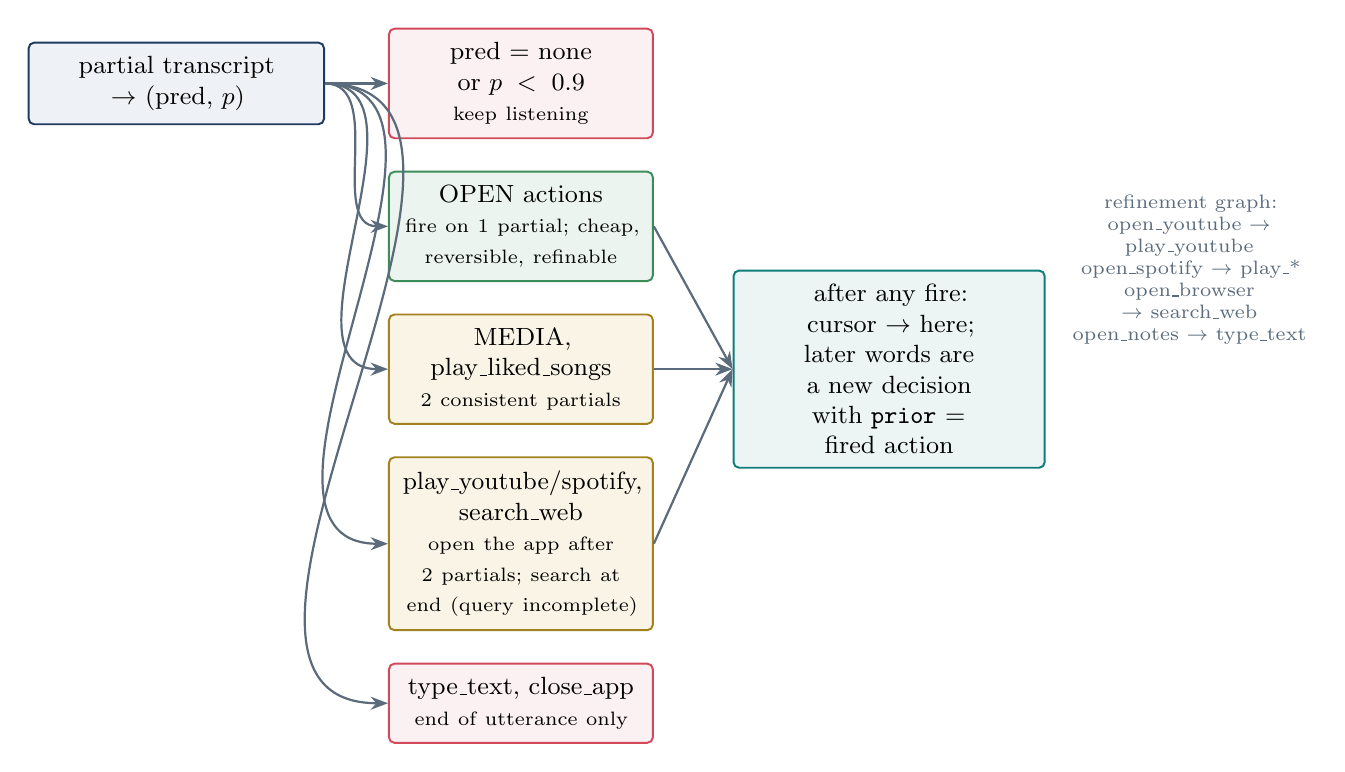
\begin{tikzpicture}[node distance=4mm]
\node[boxk,text width=34mm] (in) {partial transcript $\to$ (pred, $p$)};
\node[boxc,right=8mm of in,text width=30mm] (none) {pred = none\\ or $p<0.9$\\ \scriptsize keep listening};
\node[boxl,below=of none,text width=30mm] (open) {OPEN actions\\ \scriptsize fire on 1 partial; cheap, reversible, refinable};
\node[boxg,below=of open,text width=30mm] (media) {MEDIA, play\_liked\_songs\\ \scriptsize 2 consistent partials};
\node[boxg,below=of media,text width=30mm] (slot) {play\_youtube/spotify, search\_web\\ \scriptsize open the app after 2 partials; search at end (query incomplete)};
\node[boxc,below=of slot,text width=30mm] (def) {type\_text, close\_app\\ \scriptsize end of utterance only};
\node[boxt,right=10mm of media,text width=36mm] (res) {after any fire: cursor $\to$ here;\\ later words are a new decision\\ with \code{prior} = fired action};
\draw[arr](in)--(none);\draw[arr](in.east) to[out=0,in=180] (open.west);\draw[arr](in.east) to[out=0,in=180] (media.west);\draw[arr](in.east) to[out=0,in=180] (slot.west);\draw[arr](in.east) to[out=0,in=180] (def.west);
\draw[arr](open.east)--(res.west);\draw[arr](media.east)--(res.west);\draw[arr](slot.east)--(res.west);
\node[lbl,right=2mm of res.north east,anchor=west,text width=30mm] {refinement graph:\\ open\_youtube $\to$ play\_youtube\\ open\_spotify $\to$ play\_*\\ open\_browser $\to$ search\_web\\ open\_notes $\to$ type\_text};
\end{tikzpicture}
\caption{The class-aware commit/refine policy (\code{stream\_policy.py}, applied incrementally in the live loop).}
\label{fig:policy}
\end{figure}

\begin{table}[H]
\centering\small
\begin{tabularx}{\textwidth}{X L{46mm} R{22mm}}
\toprule
Class-aware policy, 198 actionable utterances & transcript last & transcript first \\
\midrule
Utterances with a \textbf{harmful} action (not in accepted set nor an ancestor of it) & \textbf{1} (0.5\%) --- ``clothes the notepad'', an ASR-error row & 2 \\
Final action consistent with the label & 0.985 & 0.965 \\
Mean word of first action & 3.6 & 3.6 \\
First action at or before the human commit word & 53\% & 53\% \\
Actions per utterance & 1.30 & 1.28 \\
Out-of-scope utterances (22) with a false action & \textbf{2} & 4 \\
Compound rows: residual routes to the second action, without / with \code{prior} & 20/22 / \textbf{22/22} & --- \\
\bottomrule
\end{tabularx}
\caption{Harm-oriented evaluation. The two false actions on out-of-scope speech are ``youtube is down again'' $\to$ YouTube opens at word 1 and ``my notes from the meeting \ldots'' $\to$ Notepad at word 2: prefixes that \emph{are} commands until the sentence continues. That is end-pointing, a property of language, mitigated by cheap-action-first and an undo window --- not by a better classifier.}
\end{table}

\subsection{The ASR stage}
\begin{table}[H]
\centering\small
\begin{tabularx}{\textwidth}{X R{24mm} R{24mm}}
\toprule
faster-whisper, FP16 GPU, 200\,ms chunks, re-decoding the growing buffer, synthetic speech & base.en & small.en \\
\midrule
Partial decode latency p50 / p95 & \textbf{41 / 131\,ms} & 120 / 207\,ms \\
WER vs command text / exact match & 7.8\% / 75\% & 7.3\% / 77\% \\
WER, noisy style / all other styles & 24\% / $\le$10\% & 23\% / $\le$7\% \\
Final transcript's words already stable at 50\% / 75\% of the utterance & 81\% / 97\% & 84\% / 98\% \\
Intent from ASR transcript agrees with intent from true text & \textbf{97.3\%} & 97.7\% \\
Intent accuracy from ASR / from text & 0.900 / 0.909 & 0.905 / 0.909 \\
\bottomrule
\end{tabularx}
\caption{ASR costs about one point of intent accuracy; small.en buys under one point for 3$\times$ the latency. The six disagreements are genuine mis-hearings (``quit chrome'' $\to$ ``quick crow'', ``pause'' $\to$ ``paw'').}
\end{table}

\subsection{End to end}
\begin{figure}[H]
\centering
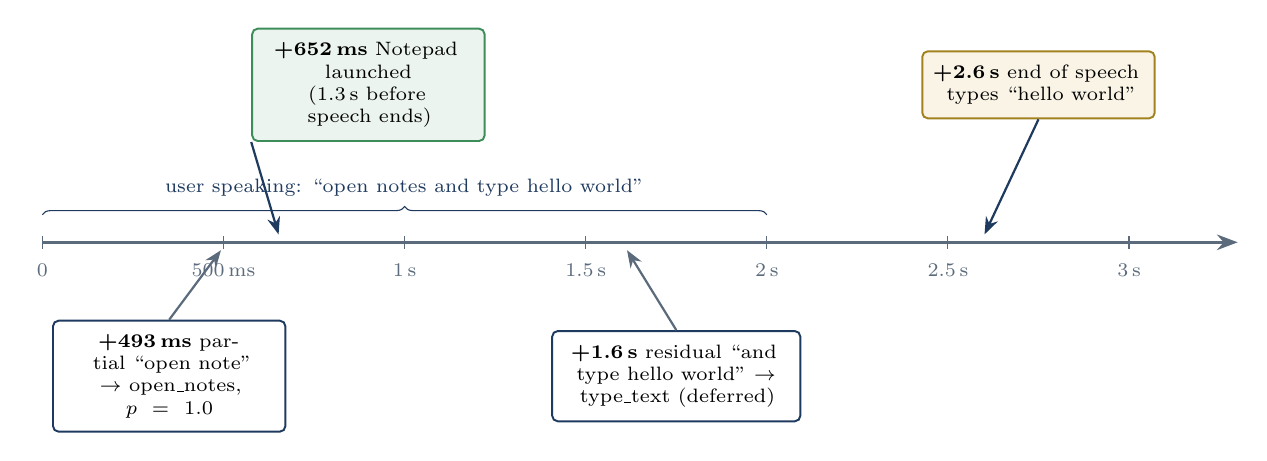
\begin{tikzpicture}[x=46mm,y=10mm]
\draw[line width=1pt,color=slate,-{Stealth}] (0,0) -- (3.3,0);
\foreach \t/\l in {0/0, 0.5/500\,ms, 1/1\,s, 1.5/1.5\,s, 2/2\,s, 2.5/2.5\,s, 3/3\,s} { \draw[color=slate] (\t,-0.08)--(\t,0.08); \node[lbl] at (\t,-0.35) {\l}; }
\draw[decorate,decoration={brace,amplitude=3pt},color=navy] (0,0.35) -- (2.0,0.35) node[midway,above=3pt,font=\scriptsize\color{navy}] {user speaking: ``open notes and type hello world''};
\node[box,font=\scriptsize,text width=26mm] (n0) at (0.35,-1.7) {\textbf{+493\,ms} partial ``open note''\\ $\to$ open\_notes, $p=1.0$};
\draw[arr] (n0.north) -- (0.493,-0.1);
\node[boxl,font=\scriptsize,text width=26mm] (n1) at (0.9,2.0) {\textbf{+652\,ms} Notepad launched\\ (1.3\,s before speech ends)};
\draw[arrn] (n1.south west) -- (0.652,0.1);
\node[box,font=\scriptsize,text width=28mm] (n2) at (1.75,-1.7) {\textbf{+1.6\,s} residual ``and type hello world'' $\to$ type\_text (deferred)};
\draw[arr] (n2.north) -- (1.614,-0.1);
\node[boxg,font=\scriptsize,text width=26mm] (n3) at (2.75,2.0) {\textbf{+2.6\,s} end of speech\\ types ``hello world''};
\draw[arrn] (n3.south) -- (2.601,0.1);
\end{tikzpicture}
\caption{Live run from audio (\code{voice\_demo.py --wav}, timings from the recording's own clock, contended GPU). The first action lands $\sim$1.3\,s before the user stops speaking; the deferred action executes with the exact slot at end of speech.}
\end{figure}

\begin{table}[H]
\centering\small
\begin{tabular}{l r l}
\toprule
Stage, per streamed word & ms & note \\
\midrule
ASR partial & $\sim$40 & base.en GPU; grows with buffer length \\
decision compute & $\sim$30 & 11 uncached tokens on the 12B Q8; 2.7\,ms/token \\
HTTP + JSON & $\sim$15 & removable with an in-process loop \\
policy + slot extraction & $<1$ & pure Python; slots regex 90/93 exact on labelled rows \\
\midrule
\textbf{word $\to$ action dispatched} & \textbf{$\sim$85} & before the next word has finished \\
\bottomrule
\end{tabular}
\caption{The measured budget. Humans read $\sim$100\,ms as instantaneous; the decision is inside that. What remains outside it is end-pointing for the deferred actions (600\,ms of silence) and OS launch time.}
\end{table}

\paragraph{What this adds over speech-to-intent engines.} Rhino/Snips-class systems have delivered 12--60\,ms on fixed intent sets since 2019. What the one-pass layer adds: an \emph{editable, zero-shot} action set (add ``open Notion'' by editing one JSON line, no retraining), a calibrated early-commit signal with a measured harm rate, multi-step decisions on the residual with a \code{prior}, and one primitive shared with the LLM fallback.

% ================================================================ 8b
\section{Head-to-head with Laya, on Laya's own benchmarks}
\label{sec:laya}

Laya (Convai Innovations, Apache-2.0) is the strongest open ``System One'' project besides SemIf and the one that claims to beat Jev. It is a different design: a bidirectional \emph{encoder} (ModernBERT-large 421M for English, mmBERT-base 322M for 100+ languages) with one \code{[MASK]} marker per option --- \code{[CLS] type+instructions [SEP] [MASK] opt$_0$ [MASK] opt$_1$ \ldots\ [SEP] state [SEP]} --- a two-layer head that scores the marker positions, and training by reinforcement learning against a proper scoring rule (log + spherical + ranked-probability score, ``RLCD''). Confidence is $1-H(p)/\log k$; one temperature per (question type, option-count bucket). It reports 33\,ms per question on a T4, 45 of 51 languages usable, ECE 0.081 after temperature refit, and 0.766 on the typed-decisions benchmark against Jev's published 0.727. Its README also states its limits plainly: the base checkpoints are near chance zero-shot on typed-decisions (0.36 vs 0.318 random), the 0.766 comes from a checkpoint fine-tuned on that benchmark's own training split, choice questions should stay under $\sim$20 options (Banking77: 0.425), and it ships over-confident.

Laya could not run Jev (no API access), so every Laya-vs-Jev number is a cross-benchmark comparison. We can do better than that here: \textbf{Laya's three checkpoints and Tez answered byte-identical rows on the same GPU} (\code{experiments/bench\_h2h.py}), using Laya's own datasets and, where it publishes one, its own protocol (MASSIVE: first 100 test rows per language, 20 options = gold + 19 sampled with seed 13, shuffled). Tez is the frozen Gemma 4 12B Q8\_0 with the one-pass letter readout, zero-shot, options first and state last; questions with more than 26 options (Banking77) are run as a chunked tournament (four chunks of $\le$20 plus ``none of these'', winners meet in a final round; five passes). Laya runs in-process with its shipped temperatures. Metrics are Laya's (accuracy, macro-F1, ECE-15, Brier, NLL, mean confidence, accuracy at 50\% coverage) plus a 2-fold out-of-fold temperature refit for every model, option-order flip rate on the first 100 rows of each choice task, and wall-clock ms per decision. Jev's numbers are third-party published and are shown only where they exist.

\begin{figure}[H]
\centering
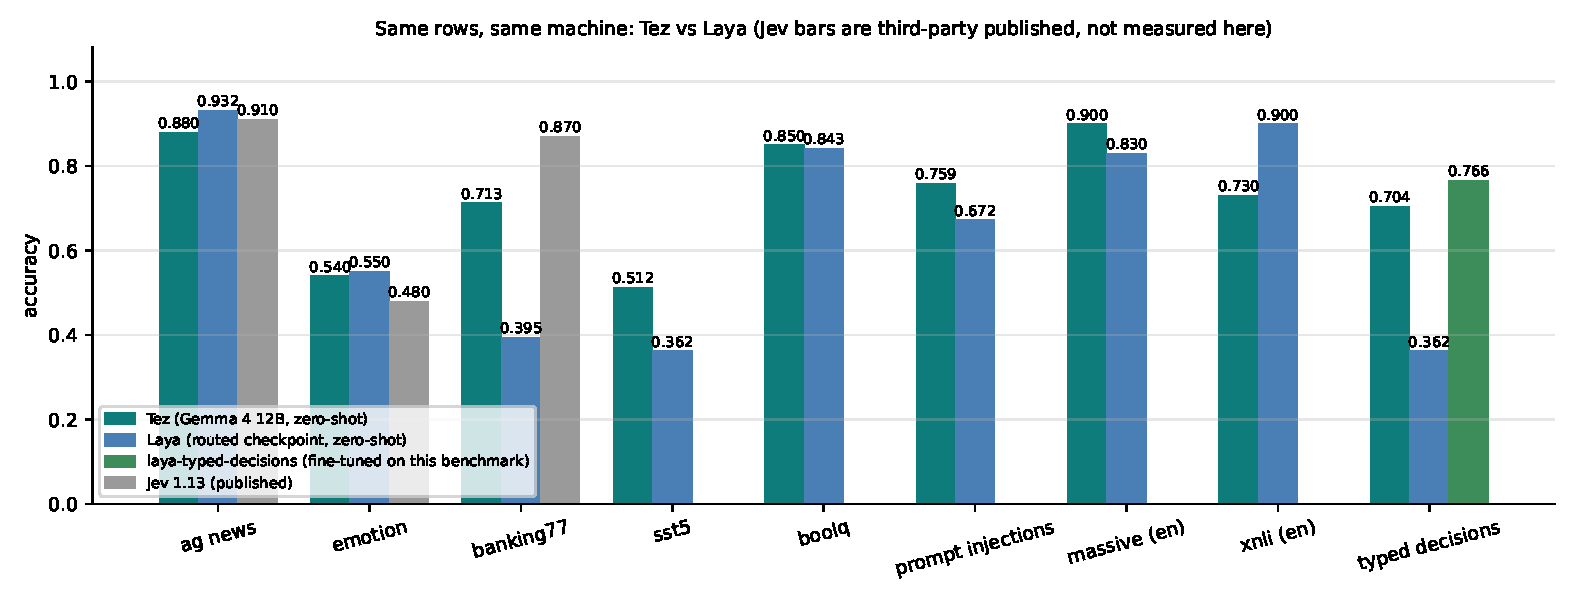
\includegraphics[width=\textwidth]{../figures/tez_vs_laya_vs_jev.pdf}
\caption{Accuracy on Laya's public datasets, same rows, same machine. ``Laya (routed)'' is the checkpoint Laya's own \code{Router} would pick (English $\to$ \code{laya}, otherwise \code{laya-multilingual}). AG News and BoolQ are in Laya's training mix.}
\label{fig:h2h}
\end{figure}

\begin{table}[H]
\centering\footnotesize
\resizebox{\textwidth}{!}{%
\begin{tabular}{l r r r r r r r r r r}
\toprule
& \multicolumn{4}{c}{accuracy} & \multicolumn{2}{c}{ECE-15 shipped $\to$ refit} & \multicolumn{2}{c}{order flip} & \multicolumn{2}{c}{ms / decision} \\
\cmidrule(lr){2-5}\cmidrule(lr){6-7}\cmidrule(lr){8-9}\cmidrule(lr){10-11}
task ($n$) & \textbf{Tez} & laya & laya-ml & laya-td & Tez & laya & Tez & laya & Tez & laya \\
\midrule
AG News (400; in Laya's training mix) & 0.880 & \textbf{0.932} & 0.948 & 0.932 & 0.11$\to$0.04 & 0.03$\to$0.03 & 0.03 & 0.00 & 65 & 39 \\
DAIR Emotion (400) & 0.540 & \textbf{0.550} & 0.487 & 0.547 & 0.43$\to$0.06 & 0.36$\to$0.07 & 0.07 & 0.06 & 60 & 36 \\
Banking77 (400, 77 options) & \textbf{0.713} & 0.395 & 0.357 & 0.388 & 0.27$\to$0.07 & 0.52$\to$0.07 & --- & --- & 589 & 56 \\
SST-5 (400, ordinal score) & \textbf{0.512} & 0.362 & 0.280 & 0.460 & 0.47$\to$0.09 & 0.29$\to$0.10 & --- & --- & 57 & 45 \\
BoolQ (400, noul; in Laya's mix) & \textbf{0.850} & 0.843 & 0.782 & 0.835 & 0.13$\to$0.03 & 0.08$\to$0.02 & --- & --- & 136 & 37 \\
prompt-injections (116, noul, held out) & \textbf{0.759} & 0.672 & 0.569 & 0.647 & 0.24$\to$0.07 & 0.31$\to$0.03 & --- & --- & 64 & 50 \\
MASSIVE intent, English (100, 20 options) & \textbf{0.900} & 0.830 & 0.710 & 0.820 & 0.09$\to$0.05 & 0.13$\to$0.09 & \textbf{0.07} & 0.18 & 174 & 45 \\
MASSIVE, macro over 11 languages & \textbf{0.885} & 0.354 & 0.524 & 0.345 & 0.10 & 0.49 / 0.30 & & & 182 & 38 \\
\quad Khmer & \textbf{0.790} & 0.000 & 0.210 & 0.050 & & & & & & \\
XNLI, English (100) & 0.730 & 0.900 & 0.860 & \textbf{0.920} & 0.26$\to$0.11 & 0.05$\to$0.05 & & & 73 & 35 \\
XNLI, macro over 10 languages & 0.699 & 0.609 & \textbf{0.794} & --- & & & & & & \\
typed-decisions (2,000 decisions) & \textbf{0.704}$^{\dagger}$ & 0.362 & 0.352 & 0.766$^{\ddagger}$ & 0.26$\to$0.05 & 0.17$\to$0.04 & & & 248 & 36 \\
\quad soft accuracy vs the teacher distribution & \textbf{0.575} & 0.331 & 0.328 & 0.471 & \multicolumn{6}{l}{Jev published: 0.727 accuracy, 0.580 soft accuracy} \\
\bottomrule
\end{tabular}}
\caption{Same rows, same GPU. $^{\dagger}$zero-shot; $^{\ddagger}$fine-tuned on this benchmark's training split (Laya's own caveat). Laya's published figures reproduce within a point or two in our harness (e.g.\ typed-decisions base 0.362 vs their 0.362, fine-tuned 0.766 vs 0.766, Khmer 0.000 vs 0.000), which validates the comparison.}
\label{tab:h2h}
\end{table}

\begin{figure}[H]
\centering
\begin{subfigure}{0.5\textwidth}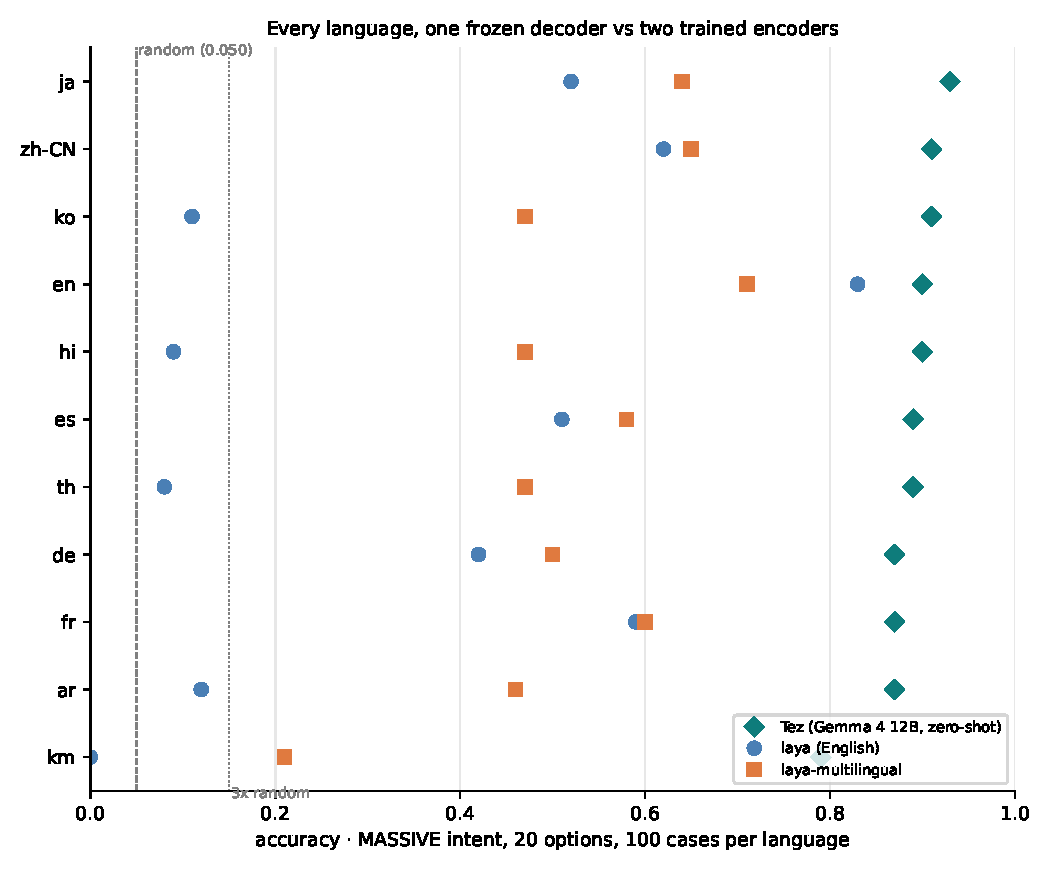
\includegraphics[width=\textwidth]{../figures/languages.pdf}\caption{MASSIVE intent, 20 options, per language.}\end{subfigure}\hfill
\begin{subfigure}{0.47\textwidth}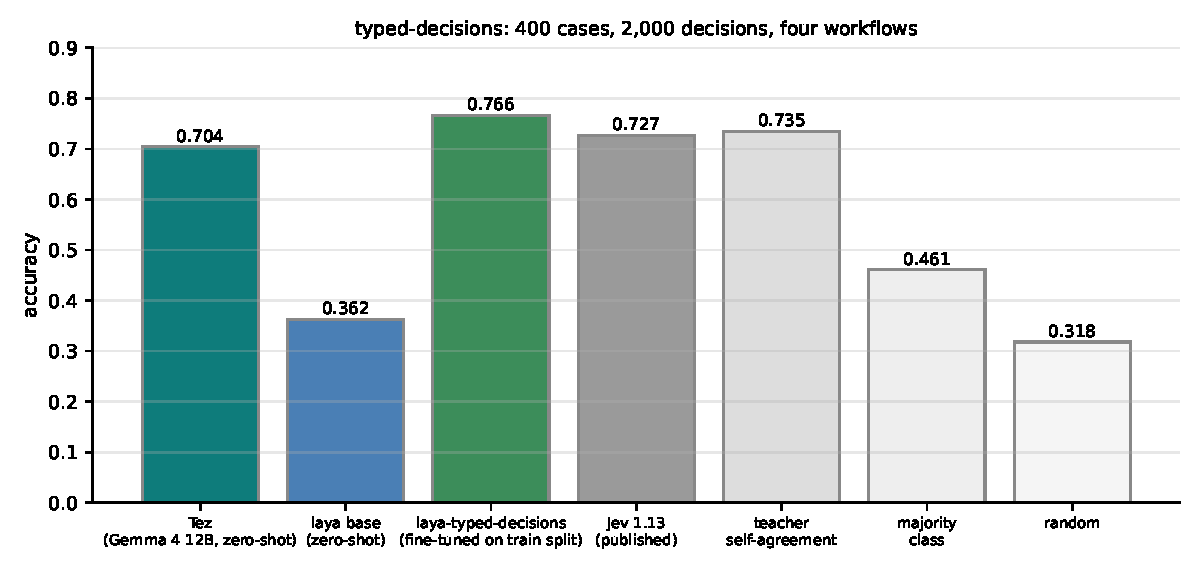
\includegraphics[width=\textwidth]{../figures/typed_decisions.pdf}\caption{typed-decisions, with Laya's reference points.}\end{subfigure}
\caption{Laya's two headline charts, redrawn with Tez on the same rows.}
\end{figure}

\begin{figure}[H]
\centering
\begin{subfigure}{0.49\textwidth}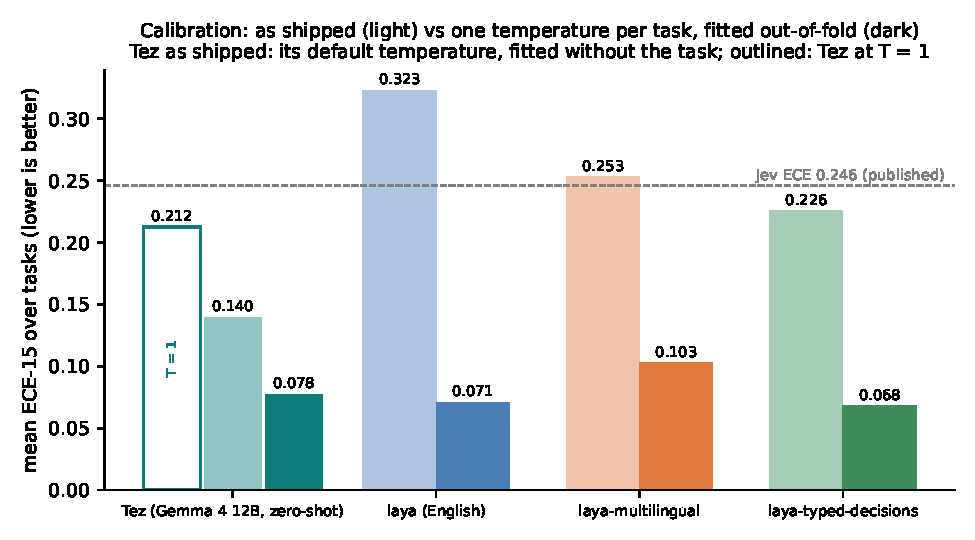
\includegraphics[width=\textwidth]{../figures/calibration.pdf}\caption{ECE as shipped vs after a per-task temperature (2-fold OOF).}\end{subfigure}\hfill
\begin{subfigure}{0.49\textwidth}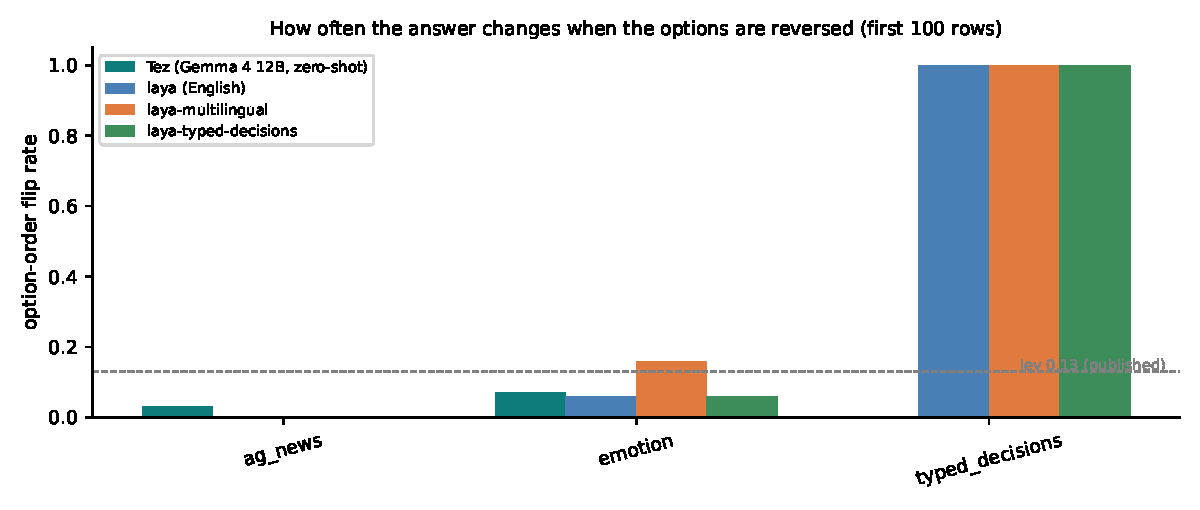
\includegraphics[width=\textwidth]{../figures/order_flip.pdf}\caption{Option-order flip rate (first 100 rows, options reversed).}\end{subfigure}
\caption{Calibration and order robustness, every model, same rows.}
\end{figure}

\paragraph{What the head-to-head shows.}
\begin{enumerate}[label=(\arabic*)]
\item \textbf{Zero-shot beats the trained encoders on six of nine English tasks} and ties one (Emotion, 0.540 vs 0.550). The exceptions are exactly the tasks in Laya's training mix or family --- AG News (0.880 vs 0.932) and NLI (XNLI-en 0.730 vs 0.900). That is the expected shape: a 400M encoder learns a task it was trained on; a frozen 12B decoder brings the knowledge to a task it has never seen.
\item \textbf{typed-decisions: 0.704 zero-shot}, against Laya's base checkpoints at 0.36 (below the 0.461 majority-class baseline), Jev's published 0.727, and 0.766 for the checkpoint fine-tuned on this benchmark's own training split. On \emph{soft} accuracy against the teacher's full distributions Tez is at 0.575 --- level with Jev's 0.580 and above the fine-tuned Laya (0.471). Nothing here was trained on the benchmark, or on anything.
\item \textbf{Multilingual is not a checkpoint problem.} One frozen model: MASSIVE macro 0.885 over eleven languages spanning six scripts, every language above 0.79, against 0.524 for Laya's multilingual checkpoint and 0.354 for its English one. Laya's Khmer result (0.000 at 0.95 confidence) reproduces exactly in our harness; Tez scores 0.790 there. Laya's answer to this is a script-detecting \code{Router} in front of two encoders; the decoder does not need one.
\item \textbf{Large option sets are a prompt-shape problem, not a ceiling.} Laya's 77-option collapse (0.395; its own explanation is the shared 192-token head budget) is not shared by the readout: a chunked tournament reaches 0.713 in five cached passes, with no embedding shortlist. Jev's published 0.870 remains ahead.
\item \textbf{Order robustness at 20 options: 0.07 vs 0.15--0.20.} Laya reports its own flip rate as worse than Jev's 0.13 and suggests more shuffling during training; the frozen 12B is already under it, and permutation averaging (\S\ref{sec:calib}) would take it lower.
\item \textbf{Calibration: as shipped, Tez is the least over-confident (mean ECE 0.212 vs 0.323 / 0.253); after one temperature per task all four land at 0.07--0.10.} Laya's calibration advantage in its README is an advantage \emph{after} refit, and refit is a lookup any model gets.
\item \textbf{Where Laya wins: speed and trained tasks.} Laya answers in 25--50\,ms in-process; Tez takes 57--250\,ms here because on these tasks the \emph{state} is the variable part and is evaluated every time (the typed-decisions states are long JSON). This is the crossover rule of \S\ref{sec:systems} in action: one state $\to$ one question favours the encoder; one state $\to$ many questions, or a constant option set with a short suffix (the voice loop, 30\,ms), favours the cached decoder. Laya also has no streaming or early-commit contract, and its own README reports moderation at 0.53 on held-out data and \code{score} as its weakest primitive (SST-5 0.372; Tez 0.512).
\end{enumerate}

\paragraph{The abstention contract, measured on 2,000 decisions.} typed-decisions is large enough to fit the conformal layer of \S\ref{sec:method} properly: split conformal on the score $1-p(\text{gold})$, Mondrian by question type, calibrated on half the \emph{cases} and evaluated on the other half (both folds, \code{experiments/conformal\_td.py}). At target coverage 90\% the sets cover 90.1\% of gold answers; Tez \emph{acts} (set of size one) on 52\% of decisions with 0.853 accuracy on those, and escalates the rest; at 95\% coverage it acts on 37\% at 0.912. The fine-tuned Laya checkpoint acts on 63\% at 0.876; Laya's base checkpoint can act on only 5\%. Zero fallbacks (empty sets) occurred. This is the contract Jev's ``confidence'' does not provide: a coverage guarantee rather than a concentration statistic.

\paragraph{Few-shot in the cached prefix: the decoder's answer to fine-tuning.} Laya's 0.766 uses the benchmark's training split through gradient updates. A cached decoder can use the same data access with none: four worked examples of the same question (state, options, answer letter) drawn from the train split are placed \emph{before} the instruction and options, so they live in the cached prefix and cost nothing per query after the first. On all 2,000 test decisions, zero-shot 0.704 $\to$ four-shot \textbf{0.725} (235 rows fixed, 194 broken, McNemar $p=0.053$), soft accuracy against the teacher distributions 0.575 $\to$ \textbf{0.583}, ECE after a per-task temperature 0.038; by primitive, \code{score} 0.642 $\to$ 0.695, \code{noul} 0.810 $\to$ 0.843, \code{choice} 0.680 $\to$ 0.645 (\code{experiments/fewshot\_td.py}; the examples share the cached prefix, so the median request evaluates 258 tokens). That puts a frozen, untrained local model level with Jev's published 0.727 accuracy on this benchmark and above its 0.580 soft accuracy, and four points below the ModernBERT checkpoint fine-tuned on the same split (0.766). This is the cheapest lever we found for domain-specific schemas: no training, no per-query latency once cached, and the examples are edited like the options themselves. The one loss --- \code{choice} --- is the same schema-drift risk the survey flags for demonstrations: examples of the \emph{same} question help, examples that merely share a workflow do not, and a per-question probe (\S\ref{sec:programme}) is the principled version.

\paragraph{``System 1.5'': a thinking budget does not help.} Gemma 4 can think before answering. Seeding its thought channel and letting it write $N$ tokens before the one-pass readout (s1-style budget forcing \cite{s1}; \code{experiments/think\_td.py}) costs $N\times$25\,ms and, on typed-decisions, buys nothing: $N=32$ is \emph{worse} (0.687 $\to$ 0.657 on 300 matched rows, $p=0.12$, \code{noul} 0.816 $\to$ 0.713 --- a truncated thought biases the readout), and $N=128$ is identical (0.753 $\to$ 0.753 on 150 rows, 10 flips each way, 4.3\,s per decision, 134 of 150 thoughts still unfinished at the budget). On the JevBench hard tier, where one family (\code{temporal\_numeric}, date and quantity arithmetic) sits at 0.133, a 64-token budget doubles that family to 0.267 but lowers the tier overall (0.703 $\to$ 0.658, $p=0.27$) and cuts \code{long\_policy} from 0.789 to 0.579: an unfinished thought over a long document biases the readout more than it informs it. On this class of decision the frozen model's first-position distribution already contains what a short deliberation would add; the literature's test-time-scaling gains are on multi-step problems, not typed judgements. The right treatment for the arithmetic family is the abstention contract --- escalate to a full reasoning pass or a tool when the set is not a singleton --- not a budget. System One stays.

\paragraph{The answer symbols do not matter at 12B.} PET-era results say bare letters are the weakest verbalizer. Re-scoring SemIf's 144 rows with digits (\code{1/2/3}) or lowercase letters instead of \code{A/B/C}: 0.947 / 0.943 vs 0.943 --- within one row. Symbol binding is not the bottleneck at this scale; it is at 3--4B (\S\ref{sec:scale}), where meaningful label words are still worth an ablation.

\paragraph{Ordinal readout: a null result.} For \code{score} questions the expected value of the distribution, rounded, is often recommended over the argmax. On SST-5 and the 800 typed-decisions score questions it changes nothing for Tez (accuracy 0.512 / 0.642 either way; MAE 0.517 vs 0.522 and 0.405 vs 0.402), and it \emph{hurts} the fine-tuned Laya checkpoint (0.724 $\to$ 0.594), whose distributions are sharper. Argmax stays.

\paragraph{Hidden-state probes: the frozen model knows more than its letter logits say.} Hidden Calibration \cite{hc} replaces the label-token readout with a linear head on the last-token hidden state. On typed-decisions we fit one logistic-regression probe per question (20 question schemas; the benchmark's 6,000 training decisions, i.e.\ the same data access as Laya's fine-tuned checkpoint) on the frozen \textbf{Qwen3.5-4B} and evaluate on the 2,000 test decisions (\code{experiments/hidden\_probe.py}). The 4B's own letter readout scores 0.490 on this benchmark. The probe on its final hidden state scores \textbf{0.772}; on the hidden state \emph{twelve layers below the top}, \textbf{0.794} (NLL 0.51 vs 1.18 for the letters; nearest-centroid alone 0.715). That is above Laya's fine-tuned ModernBERT (0.766), above Jev's published 0.727, and above the frozen 12B's zero-shot 0.704 and four-shot 0.725 --- from a model a third the size, without touching its weights, and reading a layer that lets the top third of the network be skipped. Two things follow. First, the two-stage account of \S
ef{sec:method} is confirmed directly: the decision is present in the residual stream well before it is bound to a symbol, and a probe reads it where the letter logits cannot. Second, this is the cheap, honest form of ``training'': minutes of logistic regression on frozen features, per schema, with the same labelled rows a fine-tune would need, and it composes with everything above (prefix caching, conformal sets). It is supervised, so it belongs beside Laya's 0.766 rather than the zero-shot rows. The same probe on the 12B's \emph{final} hidden state, read through llama-server's embedding endpoint (last-token pooling, L2-normalised, Q8 weights), scores 0.735 --- above the 12B's own letter readout (0.704) and its four-shot prompt (0.725), but below the 4B's intermediate layer. The intermediate layer is where the gain lives: the final layers re-shape the residual stream for next-token prediction and discard decision-relevant magnitude, exactly as the layer-wise calibration literature predicts \cite{calm}. A full sweep over all 33 layers of the 4B (\code{experiments/hidden\_probe\_sweep.py}, features cached once) makes the shape explicit: probe accuracy is 0.48 at the embedding layer (the letter readout's level), climbs through layers 14--18, plateaus at \textbf{0.79 from layer 20 to 28}, and falls to 0.772 at the top. The decision is formed at about 60\,\% of depth, so a readout there can skip the top third of the network. Three more measurements fix its practical value. \emph{Data efficiency}, rows per question: 10 $\to$ 0.669, 25 $\to$ 0.707, 50 $\to$ \textbf{0.741} (above Jev's 0.727 with 1,000 labels in total), 100 $\to$ 0.760 (Laya's fine-tuned level with a third of its data), 200 $\to$ 0.788, all 300 $\to$ 0.793 ($\pm$0.005 over seeds). \emph{Ensembling} the probe with the letter logits at one-quarter weight adds half a point (0.799). \emph{Conformal sets on the probe} at 90\,\% coverage act on \textbf{66.6\,\%} of decisions at \textbf{0.884} accuracy, against 52\,\% at 0.853 for the 12B's letter readout and 63\,\% at 0.876 for Laya's fine-tuned checkpoint: the probe is not only more accurate, it knows better when it is right. \emph{Early readout} turns the plateau into latency: truncating the frozen 4B to its first $N$ layers (\code{experiments/early\_exit\_bench.py}, 200 typed-decisions prompts, 227 tokens on average, CUDA-synchronised) costs 1.10$\times$ less at 28 layers, \textbf{1.30$\times$ at 24}, \textbf{1.54$\times$ at 20} and 1.94$\times$ at 16, while the probe read at those depths scores 0.787, 0.793, 0.790 and 0.737. Reading at layer 20--24 therefore keeps the full probe accuracy and cuts prefill by a third to a half, with no gate and no retraining; the top third of the network is spent on next-token prediction the decision does not need. The ratios are from the eager PyTorch path and transfer to a GGUF with the top layers removed.

\paragraph{Does a bigger backbone make a better probe?} No. The 12B's intermediate layers, read in-process (Gemma 4 12B, NF4 weights via bitsandbytes, first 40 of 48 layers, features z-scored per layer because Gemma's residual stream has very large magnitudes; \code{hidden\_probe\_sweep.py --load-4bit --truncate 40 --standardize}), peak at \textbf{0.787 at layer 34} (71\,\% of depth), against 0.793 for the 4B at layer 26. The 12B curve rises later and is higher only in the shallow layers. It is slightly more data-efficient (50 rows per question: 0.754 against 0.741) and slightly less accurate with more data (200 rows: 0.772 against 0.788). Conformal sets on the 12B probe act on 66.4\,\% at 0.874, the same as the 4B. Z-scoring does not explain the gap: it lowers the 4B to 0.772. The probe backbone of choice is therefore the 4B, at a third of the parameters and a sixth of the prefill.

\paragraph{Probes on Laya's public tasks.} The same recipe, one logistic-regression probe per task on 2,000 labelled training rows of the frozen Qwen3.5-4B (\code{experiments/hidden\_probe\_tasks.py}, layers 18/22/26/final, test rows identical to the head-to-head), gives: \textbf{Banking77 0.860} (layer 22; 12B letter tournament 0.713, Laya 0.395, Jev published 0.870), Emotion 0.640 (4B letters 0.468, 12B 0.540, laya-td 0.547), SST-5 0.547 (0.400 / 0.512 / 0.460), XNLI-en 0.860 (0.790 / 0.730 / 0.920), BoolQ 0.892 (0.752 / 0.850 / 0.835), and MASSIVE-en 0.850 over the \emph{full} 60-intent label space (the zero-shot rows choose among 20). The probe beats every zero-shot readout on every task, and it beats Laya's fine-tuned checkpoint on five of six; XNLI remains the encoder's. On Banking77 it comes within one point of Jev with one forward pass instead of five. These are supervised numbers and are reported beside Laya's fine-tuned checkpoint, not beside the zero-shot rows.

\paragraph{Two cheaper levers that did little.} \emph{Retrieval-narrowing} (\code{experiments/retrieval\_narrow.py}): MiniLM (22M, Apache-2.0) shortlists the Banking77 labels, then the 12B chooses among the top $k$ in one pass. Recall is 0.90 at $k{=}10$ and 0.958 at $k{=}20$; accuracy is 0.685 and 0.733 (0.738 with a ``none of these'' fallback to the tournament), against 0.713 for the tournament, at 439\,ms instead of 589\,ms. It is a small, cheap win, bounded by the letter readout's own accuracy inside the shortlist (0.76--0.80). Using the serving model's own last-token embedding as the retriever fails outright (0.025 top-1): a decoder's final state is a next-token predictor, not a sentence embedding. \emph{Option elimination} (PoE; \code{experiments/option\_elimination.py}; top-4, top-8, above-mean log-prob, 95\,\% mass, then re-score the survivors) changes accuracy by at most two points on MASSIVE-en, Emotion, AG News and typed-decisions, in both directions, and costs a second pass. The readout already concentrates its mass: the 95\,\% set keeps 1.1 options on average and loses the gold option 10--40\,\% of the time. It is recorded as a negative result.

\paragraph{Batch Calibration, the debiasing method that does work here.} Zhao et al.'s content-free correction failed (\S\ref{sec:calib}) because empty evidence legitimately selects \emph{insufficient}. Batch Calibration \cite{bc} instead estimates the option prior from the mean log-probability over a batch of \emph{real}, unlabelled inputs and subtracts it --- zero extra passes. Applied offline to every head-to-head run, evaluated out-of-fold (prior from one half, applied to the other; \code{experiments/batch\_calibration.py}): NLL falls on 30 of 33 task/model sets, often by a lot (prompt-injections 2.89 $\to$ 1.03, XNLI-th 2.18 $\to$ 1.26, SST-5 4.04 $\to$ 3.26, typed-decisions 1.75 $\to$ 1.42); accuracy moves by $+1$ to $+4$ points on XNLI and prompt-injections, is unchanged on most tasks, and drops on Khmer ($-4$) and typed-decisions ($-1$). Rule: use it for the probabilities, gate it by a held-out accuracy check per schema, and never on tiny option sets of size $<8$.

\paragraph{A negative result: the small-to-large cascade.} A FrugalGPT-style cascade --- answer with Gemma 3 4B (40\,ms) and escalate to the 12B (110\,ms) when the 4B's two orderings disagree --- reaches 0.854 on SemIf's rows at a mean 117\,ms: \emph{slower and less accurate} than the 12B alone (0.951 at 110\,ms), because the 4B is only 2.7$\times$ cheaper and disagrees on a third of rows. Gating on the 4B's raw confidence is worse still (it is confident when wrong). On this hardware the cascade is not worth building; a cascade needs a $\ge$10$\times$ cost gap and a small model that knows when it does not know (\code{experiments/cascade\_analysis.py}).

\paragraph{What Tez does that Laya does not.} Zero-shot strength on unseen schemas (an editable option set needs no retraining); one model for every language and script; large option sets by decomposition; a measured harm-rate streaming policy; permutation-disagreement as an uncertainty signal that does not rely on the model's own confidence; the constant-first prompt layout with verified KV reuse; and an audit trail (every number in this report has a manifest, a CI or a paired test). What Laya does that Tez does not, and that the roadmap should take from it: a shipped, pip-installable runtime with typed primitives and presets, the proper-scoring-rule fine-tuning recipe with a Kaggle notebook, and a multilingual benchmark over 51 languages rather than our eleven. Fine-tuning a decoder backbone on own-traffic data with the same proper-scoring objective is the obvious next experiment; it was not attempted here, so every Tez number above is a floor.

% ================================================================ 8b
\section{The probe lab: reading decisions from the middle of the network}
\label{sec:lab}

Section~\ref{sec:laya} showed that a linear probe on a mid-depth hidden state of the frozen 4B beats every zero-shot readout. That finding is not new: Hidden Calibration \cite{hc}, the MCQ knowledge--prediction gap \cite{kappa} and the decide-then-bind account \cite{twostage} all report it. This section asks the questions that make it usable on any schema: where to read, how few labels suffice and which ones, whether labels can be avoided, what can be guaranteed, how many decisions fit in one pass, and whether the result survives a new language or a new workflow. Most experiments reuse one cache: the last-token state at every layer of the frozen Qwen3.5-4B (and layers 0--40 of the 12B, NF4) for all 8,000 typed-decisions prompts, plus the letter logits (\code{experiments/probe\_lab.py}); the rest needed one extra sweep each. Two commissioned notes supplied the ideas and the closest prior work: a cross-disciplinary survey (\code{docs/research/abstract-methods-survey.md}) and a novelty check of every experiment (\code{docs/research/novelty-check.md}). Figure~\ref{fig:lab} shows every result and Table~\ref{tab:lab} summarises them; negative results are reported as prominently as positive ones.

\begin{figure}[p]
\centering
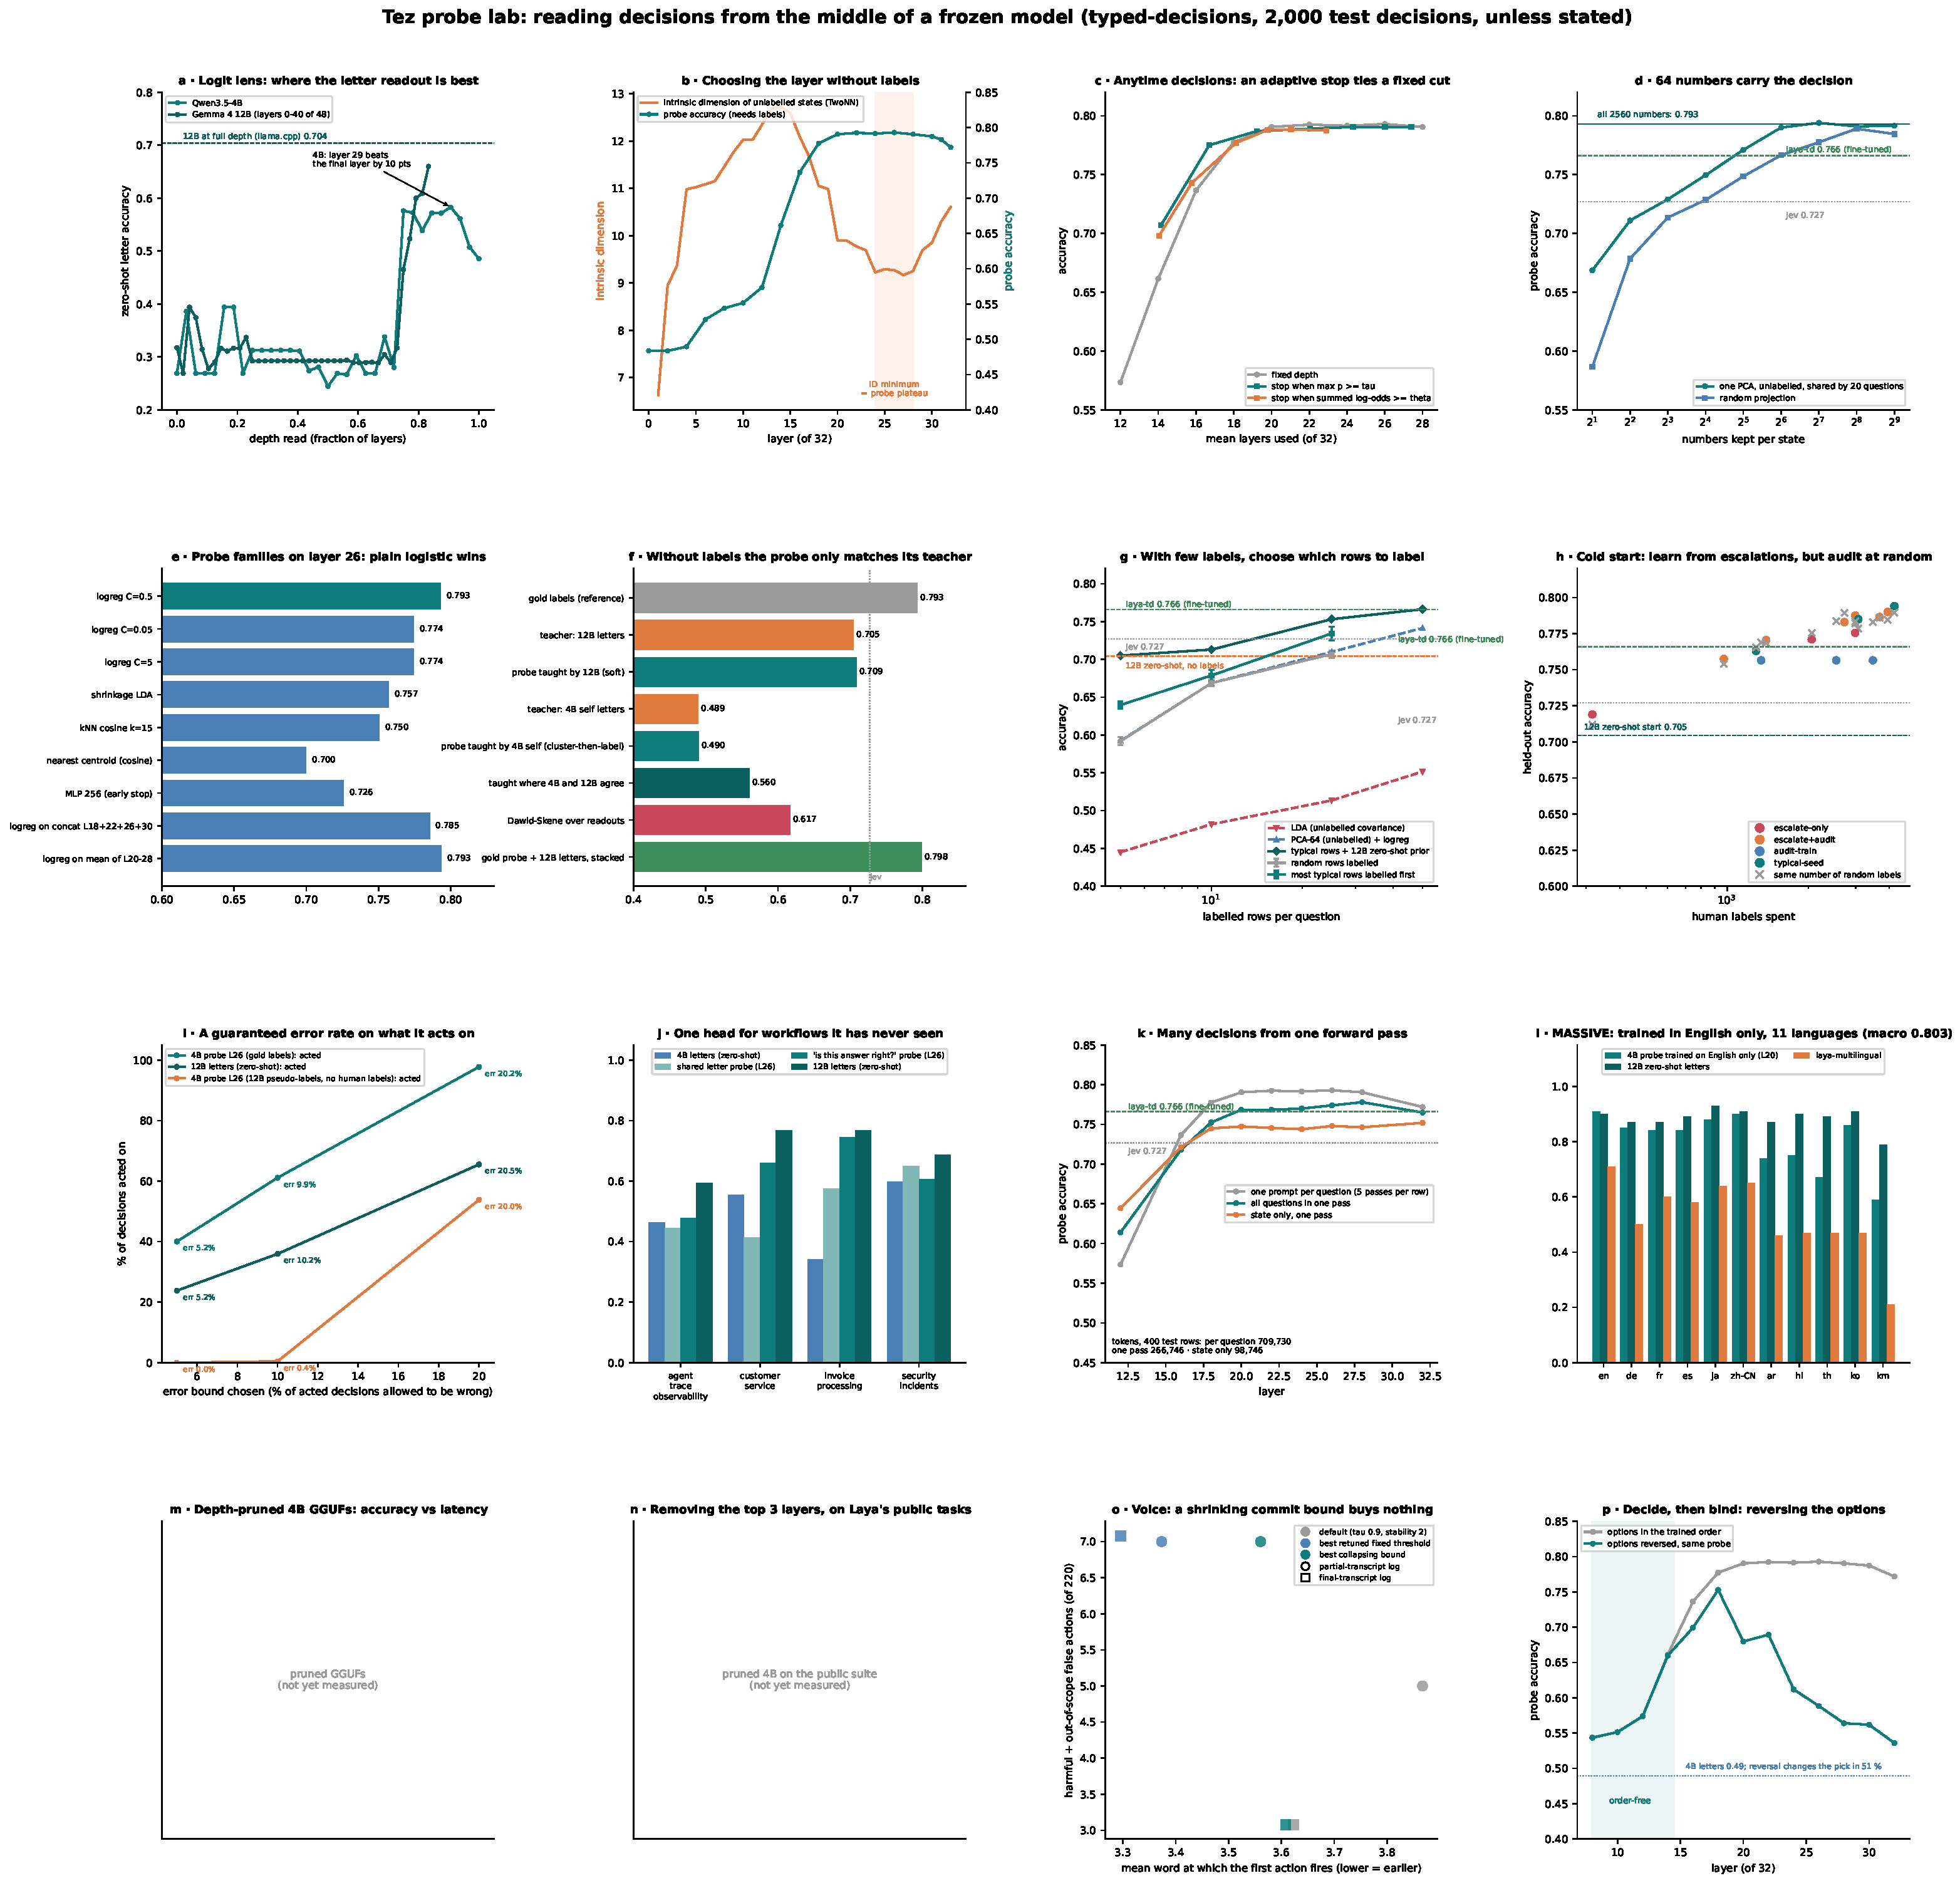
\includegraphics[width=\textwidth]{../figures/tez_lab.pdf}
\caption{The probe lab. Every panel is typed-decisions test accuracy (2,000 decisions) unless it says otherwise.}
\label{fig:lab}
\end{figure}

\begin{table}[p]
\centering\footnotesize\renewcommand{\arraystretch}{1.05}
\begin{tabularx}{\textwidth}{L{42mm} L{30mm} X L{20mm}}
\toprule
Idea & Borrowed from & Result (typed-decisions test unless stated) & Verdict \\
\midrule
Read letters at a mid layer (logit lens) & interpretability \cite{halawi} & 4B: 0.485 $\to$ 0.583 at layer 29; 12B still rising at 40/48 & \textbf{works} (model-specific) \\
Pick the layer with no labels & dynamical systems (intrinsic dimension) \cite{twonn,cheng} & dimension minimum = probe plateau (4B layers 24--28); lands on the 12B plateau too & \textbf{works} \\
DoLa layer contrast & decoding \cite{dola} & 0.523 (best) & negative \\
Reverse the options at test time & two-stage binding \cite{twostage} & order-free to layer 14; $-2.4$ at 18; $-20$ at 26 & \textbf{works} (read at 18 if options move) \\
Stop climbing when sure (SPRT / gate) & sequential testing \cite{schwartz,jazbec} & 0.787 at 19.2 layers vs static cut 0.790 at 20 & ties \\
How many numbers a decision needs & rate--distortion \cite{hernandez} & 64 numbers keep 0.790; 8 keep 0.729 & \textbf{works} \\
Reuse the code on a new workflow & transfer learning & code from 3 workflows: 0.782 on the 4th (0.789 own) & \textbf{works} \\
Label the typical rows first & active learning \cite{typiclust} & 25/question: 0.734 vs 0.707 random & \textbf{works} \\
Few labels + zero-shot prior & Bayesian updating & 50 typical/question + 12B prior: 0.766 (= Laya fine-tuned) & \textbf{works} \\
LDA with unlabelled covariance & brain--computer interfaces & 0.445--0.514 at 5--25/question & negative \\
Probe from zero-shot answers & weak-to-strong \cite{w2s} & matches its teacher (0.709 vs 0.705), never beats it & neutral \\
Dawid--Skene over readouts & epidemiology / weak supervision & 0.617 (< 12B alone) & negative \\
Stack probe + 12B letters & forecast aggregation & 0.7985 (+0.5) & small \\
Two backbones' probes together & ensembling & 0.798 (0.793 and 0.787 alone); 98\,\% right where the benchmark's labels are decisive & ceiling reached \\
Calibration of the probe & proper scoring rules & ECE 0.023 as read (12B letters 0.262; Jev published 0.246) & \textbf{works} \\
Escalate + audit, learn online & human-in-the-loop \cite{rauch} & 95\,\% automated at 0.707 (5\,\% labelled) $\to$ 50\,\% at 0.868 & \textbf{works} with a strong prior \\
Bound the error of acted decisions & multiple testing \cite{confsel} & 5\,\% bound: acts on 40\,\% at 5.2\,\% error & \textbf{works} \\
One head for unseen workflows & zero-shot heads \cite{chenhf} & 0.52 vs 0.49 letters & negative \\
Universal ``is this answer right?'' probe & truth directions \cite{truthhyper,orgad} & unseen workflows 0.622 (4B letters 0.490; 12B 0.705) & \textbf{works} \\
Select-and-copy attention heads & attention as retrieval \cite{selectcopy} & top-3 heads 0.503; heads from other workflows 0.503 & negative \\
Many decisions in one pass & batching \cite{mti} & 2.7$\times$ fewer tokens for $-1.5$ points & \textbf{works} \\
Train in English, use in 11 languages & cross-lingual transfer \cite{wendler} & 0.803 macro (Laya multilingual 0.524; 12B zero-shot 0.885) & \textbf{works} \\
Cut the served model at 24 of 32 blocks & depth pruning \cite{shortgpt} & probe 0.793 vs 0.776 at 1.5$\times$ speed; letters +10 on typed-decisions, -3.7 on the public suite (29 blocks) & \textbf{works} for probes; per task for letters \\
Read the decision through the embedding endpoint & systems & 4B-24 probe: 58\,ms at 0.793; full 4B letters 136\,ms at 0.483; 12B letters 207\,ms & \textbf{works} \\
Collapsing voice commit bound & drift-diffusion models & no policy earlier and as safe & negative \\
\bottomrule
\end{tabularx}
\caption{Every idea tried in the probe lab, where it came from, and whether it survived.}
\label{tab:lab}
\end{table}


\paragraph{Where to read.} Reading the letter logits at an intermediate layer through the final norm and the tied head (the logit lens) lifts the 4B's zero-shot accuracy from 0.485 at layer 32 to \textbf{0.583 at layer 29}; the layer was chosen on the train split, and layers 24--30 all score 0.54--0.58. The last three layers of this model spend compute to lose accuracy, the ``overthinking'' pattern of \cite{halawi} on a decision task. The 12B behaves the opposite way: its letter readout is still rising at layer 40 of 48 (0.66) and is best at full depth (0.704), so the effect belongs to the model, not to the method. DoLa's layer contrast \cite{dola} peaks at 0.523, a null that matches \cite{kappa}. The obvious label-free way to pick the lens layer, maximum confidence, fails (it picks layer 21: 0.269). A different label-free signal works for the probe. The intrinsic dimension of the unlabelled states (TwoNN \cite{twonn} on 2,000 train states per layer) rises to a peak of 12.7 at layers 13--14, falls to its minimum of 9.2--9.3 at \textbf{layers 24--28} --- exactly the probe's accuracy plateau (0.790--0.793) --- and rises again at the top, where accuracy falls. On the 12B the dimension peaks at layer 28 and falls to the last cached layer while the probe sits on its plateau, so the rule ``lowest dimension after the peak'' lands on the plateau for both models (exactly for the 4B, 1.1 points below the best layer for the 12B). The decision layers are where the representation is most compressed; \cite{cheng} report the complementary fact that the dimension peak marks the start of the abstract phase. The layer can therefore be set before a single label exists.

\paragraph{How deep to go.} Stopping per input when a per-layer probe is confident (a max-probability gate, or an SPRT-style sum of log-odds over depth) gives 0.787 at 19.2 layers on average; the static cut at layer 20 gives 0.790 at 20. The adaptive rule ties the static one and leads only at very aggressive budgets, as the early-exit literature predicts for residual streams whose layers are strongly correlated \cite{schwartz,jazbec}. The static cut is the one to ship.

\paragraph{When the options move: decide, then bind, measured across depth.} Probes are trained on prompts with the options in their usual order and predict the chosen \emph{option}, not its letter. Presenting the test options in reverse order, so that every letter now points at a different option, separates layers that carry the decision as content from layers that carry it as a position. Up to layer 14 reversal costs nothing (0.660 against 0.661); at layers 16--18 it costs 2--4 points (0.753 against 0.777 at layer 18); from layer 20 the cost grows steadily, 11 points at layer 20, 20 at layer 26 and 24 at the top. The decision is formed as content first and bound to option positions from about 60\,\% of depth, the two-stage account of \cite{twostage} measured directly. The letters themselves are far more order-bound: reversing the options changes the option the 4B's letter readout picks in 51\,\% of decisions. The practical rule: if a schema may reorder its options, read the probe at layer 18 (0.777, 2.4 points lost to reversal) rather than 26 (0.793, 20 points lost), or refit it after the edit.

\paragraph{What to read with, and how much of it.} Plain logistic regression on one layer (0.793) beats shrinkage LDA (0.757), cosine kNN (0.750), a small MLP (0.726) and nearest centroids (0.700); concatenating four layers (0.785) or averaging layers 20--28 (0.793) adds nothing, and stacking the probe with the 12B's letters adds half a point (0.7985). The decision needs very few numbers. One PCA, fitted on unlabelled states and shared by all 20 questions, keeps \textbf{0.790 with 64 numbers per state} (0.794 with 128), 0.771 with 32, and 0.729 --- Jev's published level --- with 8; random projections need about four times as many. The code also travels: a PCA fitted on the other three workflows and applied unchanged to a fourth keeps 0.782 at 64 numbers and 0.790 at 128 (0.789 and 0.793 when fitted on that workflow itself). A 64-number decision code is 40 times smaller than the state and can be learned once, from unlabelled traffic, and reused on new schemas; low-dimensional concept subspaces are known in general \cite{hernandez}, the count and the transfer for typed decisions are the new part.

\paragraph{Few labels: choose which rows a human labels, and keep the zero-shot prior.} With 5, 10, 25 and 50 labelled rows per question, labelling the most \emph{typical} rows first (the member nearest each k-means centre of the unlabelled states, as in TypiClust \cite{typiclust}) beats random rows at every budget (0.618--0.640 against 0.592 at 5; 0.733--0.734 against 0.707 at 25). Mixing that probe with the 12B's zero-shot distribution, with weight $n/(n+10)$ on the probe, is better than either: \textbf{0.753 at 25 labels per question and 0.766 at 50} --- the level of Laya's checkpoint fine-tuned on the whole train split --- starting from 0.705 with none. Borrowing the covariance from unlabelled states for LDA, a trick from brain--computer interfaces, does \emph{not} work here (0.445--0.514 at 5--25 labels): class means from a handful of rows are too noisy for a 2,560-dimensional inverse.

\paragraph{No labels at all: a probe matches its teacher, it does not beat it.} Training the probe on zero-shot answers instead of human labels is the weak-to-strong setting \cite{w2s}. With the 4B's own letters as teacher (0.489) every variant --- hard, confidence-filtered, soft, three rounds of cross-fitted self-training, cluster-then-label --- lands between 0.470 and 0.490, never above the teacher, as \cite{w2s} predicts when the student can reproduce the teacher's errors (the letter readout is itself a linear map of the same network's states). With the 12B's answers as teacher (0.705) the 4B probe reaches 0.705 with hard labels and 0.709 with soft ones: a model three times smaller, with no human label, matches the larger model's zero-shot decisions, but does not beat them. Filtering to confident teacher answers hurts (0.59--0.66: the filter keeps the easy classes), and so does combining readouts first with a Dawid--Skene label model (0.617): the weak, correlated 4B views outvote the strong one. Labels are where the gain is.

\paragraph{Cold start: begin zero-shot, escalate, learn from the escalations.} A deployment rarely starts with labels. Streaming the 6,000 train decisions through the 12B's zero-shot readout, escalating to a human whenever the current readout's confidence is below a threshold, and refitting the per-question probe (blended with the zero-shot prior) as labels arrive gives a system that improves as it runs. At threshold 0.6 it escalates 5\,\% of decisions and automates the other 95\,\% at 0.707. Adding a random audit slice of 5--10\,\% of traffic --- labels that are \emph{not} chosen by uncertainty --- lifts the automated accuracy to 0.75--0.78 on 77--84\,\% of traffic; at threshold 0.8 it automates half the traffic at 0.868, and the whole stream (human answers counted as correct) reaches 0.93. The probe learned this way ends where one trained on the same number of random labels ends ($\pm$0.5 points). The prior matters: starting instead from the 4B's own letters (0.489), labels gathered only from uncertain decisions train a \emph{worse} probe than random labels at the same budget (0.678 against 0.746 with 20\,\% labelled), because escalations are a biased sample \cite{rauch}. Start from the strongest zero-shot readout available, and keep an audit slice.

\paragraph{Guarantees: bound the error rate of what it acts on.} Conformal selection \cite{confsel} turns any readout into a policy with a guarantee: compute a conformal p-value for ``this decision is wrong'' against a calibration set and act on the decisions that Benjamini--Hochberg selects. At a 5\,\% bound the gold-label probe acts on \textbf{40\,\%} of decisions with a realised error of 5.2\,\% among them (50 random calibration splits; worst split 9.6\,\%); at 10\,\% it acts on 61\,\% with 9.9\,\% errors. The 12B's zero-shot readout acts on only 24\,\% at the same 5\,\% bound. The probe trained on 12B pseudo-labels has the right accuracy but not the right confidence: it cannot act on anything at 5\,\%, because it learned to imitate its teacher's confidence rather than its own correctness --- a second reason to prefer real labels.

\paragraph{Where the remaining errors are.} Every supervised route in this section converges on 0.79--0.80: probes on two different backbones (0.793 and 0.787), their ensemble (0.798), and stacking with the 12B's letters (0.7985). The benchmark explains why. Its gold label is the argmax of a soft distribution over the options (they agree on 98.5\,\% of test decisions), and that distribution is often split: on the quarter of decisions where it puts at least 0.8 on one option the probe is right \textbf{98\,\%} of the time (the 12B's letters 95\,\%), at 0.6--0.8 it is right 85\,\%, at 0.5--0.6 71\,\%, and on the fifth of decisions where no option reaches 0.5 it is right 56\,\%. The readout has reached the benchmark's resolution: most of what remains is disagreement the benchmark itself encodes.

\paragraph{Calibration comes with the labels.} A logistic probe is fitted with a proper scoring rule, so its probabilities are calibrated as they come out: expected calibration error 0.023 for the gold-label probe and 0.028 for the 12B prior plus 50 typical labels per question, against 0.262 for the 12B's raw letters (0.067 only after a fitted temperature) and 0.246 published for Jev. The labels also go where the zero-shot readout is weakest: ordinal \emph{score} questions gain the most (0.642 for the 12B's letters, 0.752 for the probe), yes/no questions the least (0.812 to 0.873).

\paragraph{Many decisions from one forward pass.} Today every question is its own prompt (question and options first, state last), so a row with five questions pays for the state five times. Putting the state first and all five questions after it, each ending in ``Answer $n$:'', and reading each decision at its own marker takes 400 passes and 266,746 tokens for the 400 test rows instead of 2,000 passes and 709,730 tokens --- \textbf{2.7 times fewer tokens} --- and the probes reach 0.778 (layer 28) against 0.793, a cost of 1.5 points. The cost is not interference: questions two to five move between $-3.7$ and $+3.0$ points against their separate prompts, so a later question is not hurt by the unanswered ones before it. It sits in the first question ($-7$ to $-10$ points), the one read straight after the state without knowing what will be asked (question and position are confounded here, because the dataset fixes the order). The zero-shot letters read at the markers even improve slightly (0.522 against 0.490). A pass over the state alone, one vector per row read by five probes, costs 7.2 times fewer tokens and 4.1 points (0.752), the known price of an embedding that does not see the question \cite{instructor}. Multi-question prompting with generated answers is known to be efficient \cite{mti}; reading several typed decisions at markers without generating, and measuring what each question loses, is the new part.

\paragraph{A new language without new labels.} A MASSIVE \cite{massive} intent probe trained on 2,000 English rows only (all 60 intents, frozen 4B) and applied unchanged to the head-to-head rows of eleven languages (20 options, Laya's protocol) reaches \textbf{0.803 macro} at layer 20 --- against 0.524 for Laya's multilingual checkpoint and 0.885 for the 12B's zero-shot letters, a model three times larger --- and against 0.695 for the same 4B's own zero-shot letters on those rows (the uncut 4B GGUF in the head-to-head harness): labels in one language lift the other ten, in every language but Thai, where the two tie. The transfer follows the language's distance from English: within 1--5 points of the 12B for German, French, Spanish, Japanese, Chinese and Korean, 13--22 points below for Arabic, Hindi, Thai and Khmer (0.59). It is also sharply layered: at layer 18 the probe already reads English (0.82) but the other languages average 0.53; at layer 20 they jump to 0.80, and the transfer decays towards the top (0.767 at layer 32). Mid-depth decoder states carry a largely language-independent decision \cite{wendler}, so a probe trained once in English serves languages it has no labels in, provided it is read where that shared state forms --- which here is the start of the typed-decisions plateau, not its end. Confidence probes are known to transfer across languages \cite{shareddoubt}; an intent probe on a decoder, per language and per layer, is the new data point.

\paragraph{One head for workflows it has never seen.} Per-question probes need that question's labels. Three question-agnostic heads were tested leave-one-workflow-out (trained on three workflows, scored on the fourth; four folds). A single probe that predicts the answer's letter position from the state reaches 0.778 on familiar workflows but only \textbf{0.521} on an unseen one, against 0.490 for the 4B's own letters, as a public bilinear-head result predicted \cite{chenhf}. A universal ``is this answer right?'' probe does much better. The frozen 4B reads the standard prompt and is made to answer with each option's letter in turn (one extra token per option on the cached prompt); a single logistic probe on the hidden state at that forced answer token, trained across questions, scores each option. On unseen workflows it reaches \textbf{0.622} at layer 26 (0.478 to 0.746 per workflow), 13 points above the 4B's letters and within 2 points of the 12B on invoice processing. It peaks at mid-depth like everything else (0.534 at the top layer). Truth directions are known to generalise when they are trained on many datasets \cite{truthhyper} and to fail across datasets when they are not \cite{orgad}; with only three training workflows the answer here is in between, and it is the best way found to decide on a new schema without its labels short of the 12B's zero-shot readout (0.705). A third head needs no training beyond choosing attention heads: the select-and-copy readout \cite{selectcopy,wiegreffe}, which reads which option the answer position attends to in Qwen3.5's eight full-attention layers. Summing the three best heads (attention to the option letter) gives 0.503 on familiar workflows and 0.503 with heads chosen on the other three workflows: the level of the 4B's own letters (0.490). The gains reported for English multiple-choice QA do not carry over to this hybrid model and these decisions.

\paragraph{Cut the model where the decision is made.} If the top layers add nothing to the decision, they need not run. \code{experiments/gguf\_truncate.py} keeps the first $N$ blocks of the Q8 GGUF plus the output norm and head, so llama.cpp's letter logits become the logit lens at layer $N$ and its \code{/embedding} endpoint returns the normed layer-$N$ state for a probe. For the probe the cut is a clean win: at \textbf{24 of 32 blocks} (3.53 instead of 4.48\,GB) a probe on the served state scores 0.793 against 0.776 for the full model, at 58 instead of 84\,ms per request (1.5$\times$; p50, prompt caching off); at 20 blocks it still holds (0.787). For the zero-shot letters the cut is task-dependent. On typed-decisions the 24-block model's letters score 0.580 against 0.483, 1.3$\times$ faster --- the logit-lens gain made deployable. Across Laya's public suite, though, the 29-block cut \emph{lowers} zero-shot letter accuracy by 3.7 points on average (20 of 28 task and language rows worse, 8 better; MASSIVE -9, BoolQ -14, typed-decisions +10). Across Laya's public suite, though, the 24-block cut \emph{lowers} zero-shot letter accuracy by 17.4 points on average (25 of 28 task and language rows worse, 2 better; MASSIVE -28, BoolQ -27, typed-decisions +10). The letters need the top layers for short inputs with many options, and are hurt by them on long structured states. So the cut is a serving optimisation for probes, and a per-task decision for letters, to be validated on the target task before it ships. Layer pruning with little loss is known \cite{shortgpt}; locating the cut from probe measurements, and finding that it can raise a decision model's zero-shot accuracy on one task family while lowering it on others, is the new part. (Prompt caching is off because llama.cpp b11100 crashes on partial prefix reuse with this hybrid architecture; a cut model sometimes predicts end-of-sequence first, so the harness re-reads the letters with that token suppressed.)

\paragraph{Where the latency goes.} The same 100 prompts, one server at a time, caching off, 3 warm-up requests: on the 24-block 4B an \code{/embedding} request (the probe's input) takes 58\,ms at p50 and a one-token \code{/completion} 112\,ms without log-probabilities and 104\,ms with the top-200 the letter readout needs; on the full 4B 84, 128 and 136\,ms; on the 12B 172, 155 and 207\,ms. On the 4B, asking for the log-probabilities costs little and the completion path itself costs 45--55\,ms more than the embedding path; on the 12B the top-200 log-probabilities add about 50\,ms and the embedding path saves nothing. So on this hardware the most accurate readout of the 4B is also the fastest: the probe on the 24-block model decides in 58\,ms at 0.793, the full model's letters in 136\,ms at 0.483, and the 12B's letters in 207\,ms at 0.705. (When the constant part of the prompt can be cached and only a few tokens are new, as in the voice layout of \S\ref{sec:voice}, the 12B decides in 30--45\,ms; the hybrid 4B cannot use prefix caching in this llama.cpp build.)

\paragraph{Streaming voice: a collapsing bound buys nothing.} A drift-diffusion observer commits against a bound that shrinks as evidence arrives. Replacing the fixed threshold of \S\ref{sec:voice} with $\mathrm{thr}(k)=f+(c-f)e^{-(k-1)/T}$, choosing $(c,f,T)$ on one half of the 220 utterances and scoring the other half, gives no policy that is both earlier and as safe as the default: the best collapsing bound and the best retuned fixed threshold both fire about half a word earlier at the cost of two more harmful actions out of 198. The default stays.

\paragraph{A recipe that carries to any schema.} Taken together, the lab gives a procedure that needs nothing specific to typed-decisions:
\begin{enumerate}[leftmargin=*,itemsep=1pt]
\item Pick the reading layer from unlabelled traffic: the minimum of the intrinsic dimension after its mid-network peak.
\item When a probe reads the state, serve the model cut at the start of that plateau (Qwen3.5-4B: 24 of 32 blocks): smaller and faster at the same accuracy. Cut for the zero-shot letters only after checking the target task. If a schema's options may be reordered, read the probe below the binding layers (layer 18 here).
\item Start from the strongest zero-shot readout available and act only under a conformal error bound; escalate the rest.
\item Spend the first labels on the most typical rows, then on escalations plus a random audit slice; blend the probe with the zero-shot prior with weight $n/(n+10)$.
\item Store 64 numbers per state (a PCA learned once, on unlabelled traffic); it transfers across workflows.
\end{enumerate}
What did not survive: probes that beat their own teacher without labels, label models over weak readouts, uncertainty-only labelling from a weak prior, DoLa, adaptive depth, question-agnostic heads on unseen workflows, and a collapsing voice bound.

% ================================================================ 8c
\section{Research programme: what the literature says to try next}
\label{sec:programme}

Three commissioned literature surveys (verified arXiv and Hub ids; full text in \code{docs/research/}) were reduced to the following ranked programme. Items already measured in this report are marked.

\begin{table}[H]
\centering\small
\begin{tabularx}{\textwidth}{L{34mm} X L{30mm} L{26mm}}
\toprule
Lever & Mechanism and source & Expected gain here & Status \\
\midrule
Few-shot in the cached prefix & worked examples of the same question before the options; AdapShot 2605.03644, many-shot ICL 2404.11018 & +5 pts on schema-specific questions & \textbf{measured}: 0.615 $\to$ 0.665 \\
Batch Calibration & subtract the batch-mean log-probability per option; 2309.17249 & NLL, +1--4 pts on NLI & \textbf{measured} \\
Conformal act/escalate & Mondrian split conformal on $1-p$; 2107.07511, MCQ conformal 2508.05544 & coverage guarantee & \textbf{measured} \\
Thinking budget (System 1.5) & seed the thought channel, stop at $N$ tokens; s1 budget forcing 2501.19393 & accuracy vs $N\times$25 ms & \textbf{measured}: null at 32 and 128 tokens, negative on JevBench hard at 64 \\
Verbalizer choice & digits / lowercase / label words instead of \code{A..P}; PET 2001.07676, ABCD 2602.17445 & $\pm$1--3 pts, calibration & \textbf{measured}: no effect on SemIf \\
Hidden-state probe & linear head on the answer-position hidden state; Hidden Calibration 2406.16535, LinC 2401.12406, judge probes 2512.22245 & +20--50 \% relative in the paper; typed-decisions 0.70 $\to$ 0.75+ & \textbf{measured}: 0.794 on frozen Qwen3.5-4B (layer $-12$); 12B mid-depth 0.787 (layer 34/48), final 0.735 \\
Order-invariant attention & options as a set via position ids; RoToR 2502.08662, PINE 2407.01100 & 6-permutation gain at 1$\times$ cost & custom attention; not yet \\
Option elimination & drop options below the mean log-prob and re-score; PoE 2310.15575, 2501.15175 & +2--5 pts on 20--77 options & \textbf{measured}: within $\pm$2 pts on four tasks; negative \\
Retrieval-narrowed labels & embed labels + demos, top-$k$ then decide; 2309.10954, RAC 2501.12332 & Banking77 0.71 $\to$ 0.80+ & \textbf{measured}: 0.738 at $k{=}20$, 1.1 passes, 439\,ms; the probe reaches 0.860 \\
State-as-prefix layout & many questions on one state share the KV; RadixAttention 2312.07104, Hydragen 2402.05099 & 5--10$\times$ per question & exact; layout only \\
Depth pruning + probe & remove 20--30 \% of layers, recalibrate; ShortGPT 2403.03853, 2604.24938 & 1.25--1.4$\times$ prefill & \textbf{measured}: 1.30$\times$ at 24 of 32 layers, 1.54$\times$ at 20, probe accuracy unchanged (\S\ref{sec:laya}) \\
Early exit with a KL gate & entropy-gated exit at 60--80 \% depth; SimExit 2507.17618, UAT 2509.23666, tuned lens 2303.08112 & 1.15--1.4$\times$ & \textbf{measured} without a gate: fixed exit at 62 \% depth is free of accuracy loss for the probe \\
Alternative backbones & Gemma 4 26B-A4B QAT-Q4 (82.6 MMLU-Pro at 4B active), Qwen3.5-9B Q8 & +3--5 pts at equal latency & \textbf{Qwen3.5-9B measured}: SemIf 0.912 (0.863--0.955), perturbations 0.868 with 8\% reversal flips, typed-decisions 0.622, 92\,ms --- below the 12B on every axis except VRAM; 26B-A4B not yet \\
Open-teacher distillation & proper-scoring-rule LoRA from frozen Qwen3.8-27B soft labels (reflex, JevBench \#5) & calibration 72 $\to$ 80+ & later; never Jev \\
\bottomrule
\end{tabularx}
\caption{The programme, ranked by expected gain per unit of engineering, from the three surveys.}
\end{table}

\paragraph{Where Tez sits on JevBench.} The independent JevBench v1.3 leaderboard (534 held-out decisions, 41 systems) has Jev at 74.4, SemIf at 73.1, djev (diffusion readout) at 73.0, a 12B-Q8 GGUF server at 71.2, and every encoder-head system --- including Laya at 54.4 --- collapsing on its hard tier. The 72/48/111 public items scored with the leaderboard's own formulas (\code{experiments/bench\_jevbench.py}, Gemma 4 12B Q8 at 8k context): original tier accuracy 0.944, chance-corrected intelligence 91.9, ECE 0.053, paraphrase-pair consistency 0.944, 53\,ms median; easy tier 1.000 / 100; \textbf{hard tier 0.703 / 55.2}, ECE 0.256, 466\,ms on states up to 3.9k tokens. Weighted with the leaderboard's tier weights (no judge tier is public) that is an intelligence of 78.2 --- indicative only, since the headline uses held-out items. Every hard-tier family is at 0.67--1.0 except \code{temporal\_numeric} at 0.133 (2 of 15): date and quantity arithmetic, which one forward pass cannot perform and which is the natural target for the thinking budget that was useless on typed-decisions (\S
ef{sec:laya}). Qwen3.5-9B scores 94.0 / 100 on the two easy public tiers, which says those tiers do not discriminate. The calibration axis, where every open decoder trails Jev by 10+ points, is the one the conformal and Batch-Calibration layers above are aimed at.

% ================================================================ 9
\section{The open landscape and what would make this the best open one}
\label{sec:landscape}
\begin{table}[H]
\centering\small
\begin{tabularx}{\textwidth}{l l l X}
\toprule
Project & Base & Licence & What it does not do \\
\midrule
SemIf & Qwen3.5-4B frozen, logit read & MIT & multi-label, abstain, batch API, debiasing, built-in calibration, streaming \\
Laya & ModernBERT-L 421M / mmBERT 322M, RLCD & Apache-2.0 & zero-shot near chance on typed-decisions; $>$20 options; 512/1024 ctx; no streaming (measured head-to-head in \S\ref{sec:laya}) \\
openJev-verdict-2.0 & ModernBERT 150M & NOASSERTION & 512 ctx; 48\% on TypeSafe's public evals \\
djev & DiffusionGemma 26B-A4B & Apache-2.0 & needs 24\,GB; calibration 65.4 \\
decider & Qwen3.5-2B SFT+RL & Apache-2.0 & hard tier 0.459; English only \\
\bottomrule
\end{tabularx}
\caption{Nobody ships: an abstain option with its own calibration; multi-label; a published $p_\text{correct}$ head fitted on a published set; order-robust options as a feature (worth +10 points on a 4B); a decision-log format; a streaming/early-commit contract; a benchmark with runtime option sets. That list is the product.}
\end{table}

\paragraph{The bar.} No independent, contamination-resistant benchmark for this class exists yet; JevBench is closest but has LLM-written ground truth and an assumed latency for self-hosted models. This report's numbers are on SemIf's public fixtures and are a reproduction, not a leaderboard. The scorecard to adopt: balanced accuracy with group-bootstrap CIs and \emph{paired} tests; Brier and NLL primary; flip rates with Wilson CIs; AUGRC and accuracy-at-coverage; latency with \code{prompt\_n} logged, fresh and cached; determinism across runs; a private human-authored hold-out hashed before the first checkpoint exists.

% ================================================================ 10
\section{Architecture and roadmap}
\begin{figure}[H]
\centering
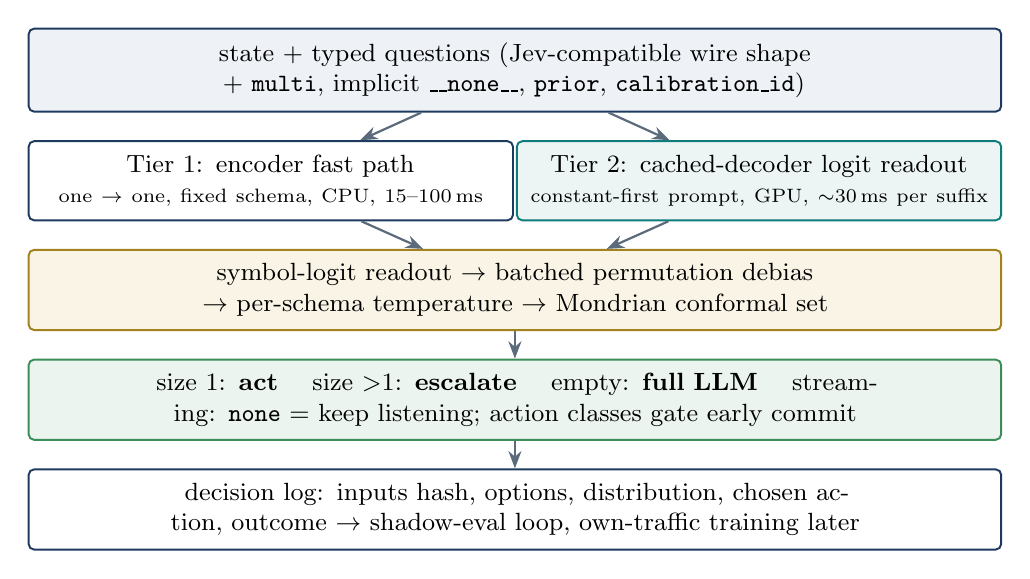
\begin{tikzpicture}[node distance=3.5mm]
\node[boxk,text width=120mm] (in) {state + typed questions (Jev-compatible wire shape + \code{multi}, implicit \code{\_\_none\_\_}, \code{prior}, \code{calibration\_id})};
\node[box,below=of in,text width=58mm,xshift=-31mm] (t1) {Tier 1: encoder fast path\\ \scriptsize one $\to$ one, fixed schema, CPU, 15--100\,ms};
\node[boxt,below=of in,text width=58mm,xshift=31mm] (t2) {Tier 2: cached-decoder logit readout\\ \scriptsize constant-first prompt, GPU, $\sim$30\,ms per suffix};
\node[boxg,below=of t2,text width=120mm,xshift=-31mm] (cal) {symbol-logit readout $\to$ batched permutation debias $\to$ per-schema temperature $\to$ Mondrian conformal set};
\node[boxl,below=of cal,text width=120mm] (act) {size 1: \textbf{act} \quad size $>$1: \textbf{escalate} \quad empty: \textbf{full LLM} \quad streaming: \code{none} = keep listening; action classes gate early commit};
\node[box,below=of act,text width=120mm] (log) {decision log: inputs hash, options, distribution, chosen action, outcome $\to$ shadow-eval loop, own-traffic training later};
\draw[arr](in)--(t1);\draw[arr](in)--(t2);\draw[arr](t1)--(cal);\draw[arr](t2)--(cal);\draw[arr](cal)--(act);\draw[arr](act)--(log);
\end{tikzpicture}
\caption{Two tiers, one contract. v1 is a harness around a frozen model; the evidence says post-hoc calibration is enough and that the frozen 12B (or a 4B with batched permutations) already reproduces and exceeds the published open baseline.}
\end{figure}

\begin{enumerate}
\item Backbone by symbol-binding screen (Gemma 4 12B passes; Q8\_0 for calibration-grade mass; a 4B with batched permutation averaging is the budget option, within noise on this data).
\item Readout at the template's exact answer position with single-token slots; \code{n\_probs} large enough for every letter; top-k always logged.
\item Six-ordering permutation averaging in one batch; PriDe on a traffic slice once volume allows; never content-free correction on option sets with an abstain answer.
\item Per-schema out-of-fold temperature, then Mondrian conformal for the act / escalate / fall-back contract; publish risk--coverage.
\item Prompt layout as part of the schema: constant first, variable last, \code{prior} for multi-step episodes; cache reuse verified by \code{prompt\_n}.
\item Decision log and shadow-eval loop; sample auto-acted cases to humans too, not only escalations.
\item Only then, optionally: LoRA on the \emph{base} model with a proper scoring rule on label-restricted logits, permutation-augmented, gated on an OOD hold-out. Never on Jev outputs; never on a benchmark's public tier that is reported.
\end{enumerate}

% ================================================================ 11
\section{Audit and limitations}
\label{sec:audit}
\begin{table}[H]
\centering\small
\begin{tabularx}{\textwidth}{X l X}
\toprule
Finding on the first draft & Severity & Resolution \\
\midrule
Balanced accuracy keyed on gold \emph{position} instead of option \emph{id} & \textbf{high} & fixed; all tables regenerated (Q8 0.953$\to$0.943, Q4 0.932$\to$0.918, Gemma 3 0.665$\to$0.646, Llama 0.458$\to$0.358) \\
``12B beats the published baseline by 14 points'' framed as a method effect & medium & SemIf lists a 27B at 0.958; 4B + permutations is within noise of the 12B \\
Q4 vs Q8 difference stated as a result & medium & McNemar $p=0.25$; reported as not significant \\
No confidence intervals on flip rates & medium & Wilson intervals; ``0/36'' bounds $\le$9.6\% \\
Labels described as authored & low & stated as model-reviewed \\
System text folded into the user turn & low & native system-turn rendering re-scored: 1 row of 144 changes \\
``$\sim$110\,ms floor / no prefix reuse'' & \textbf{high} & sliding-window cache; \code{--swa-full}; 30\,ms per word measured \\
Determinism unverified & low & three runs byte-identical \\
\bottomrule
\end{tabularx}
\caption{What the audit found and what changed.}
\end{table}

\paragraph{Limitations.} $n=144$ decisions and 36 perturbation pairs: CIs are wide and several comparisons are underpowered. The voice data is self-authored and the audio is synthetic, so ASR error is a lower bound and field noise will be worse; the out-of-scope set is small (22). Jev itself was not measured on these rows (its terms and its hosted-only access make a like-for-like local comparison impossible); comparisons with Jev are on independent public numbers only. The compound-command labelling convention (first verb as the gold intent) makes strict accuracy on that style look worse than the behaviour is; the accepting and residual metrics are the meaningful ones. Timings are from one laptop GPU and one engine build.

\section{Conclusion}
The one-pass readout is a small idea with a large surface: it turns any local instruction-tuned decoder into a typed decision function with a distribution attached, and the properties that matter --- accuracy, order robustness, calibration, latency --- are all measurable and, on this evidence, all engineerable without training. A frozen 12B reproduces and exceeds the published open baseline; the cheapest accuracy in the stack is permutation averaging, not scale; the cheapest latency is prompt layout, not a smaller model; and the piece nobody ships --- the abstention and early-commit contract --- is what turns the distribution into an action policy that opens the notes app while you are still asking for it.

The probe lab adds the second half of the recipe. Read the decision where the network has formed it and before it binds it to a letter; pick that layer from unlabelled traffic; start from the strongest zero-shot readout, act under a conformal bound, and spend the first labels on the most typical rows. Everything past that point on this benchmark is disagreement the benchmark itself encodes.

\begin{thebibliography}{99}\small
\bibitem{semif} T.~Lee. \emph{SemIf}, github.com/TheoLeeCJ/SemIf, MIT, Sept.~2026.
\bibitem{mcsb} J.~Robinson, D.~Wingate. Leveraging large language models for multiple choice question answering. arXiv:2210.12353.
\bibitem{twostage} Wong, Nouwen, Gatt. Two-stage symbol binding in multiple-choice answering. arXiv:2601.03914.
\bibitem{pet} T.~Schick, H.~Schütze. Exploiting cloze questions for few-shot text classification. arXiv:2001.07676.
\bibitem{lmbff} T.~Gao, A.~Fisch, D.~Chen. Making pre-trained language models better few-shot learners. arXiv:2012.15723.
\bibitem{sfc} A.~Holtzman et al. Surface form competition. arXiv:2104.08315.
\bibitem{zhao} Z.~Zhao et al. Calibrate before use. arXiv:2102.09690.
\bibitem{pride} C.~Zheng et al. Large language models are not robust multiple choice selectors (PriDe). arXiv:2309.03882.
\bibitem{leeson} Lee, Son. Position bias grows with option count. arXiv:2604.14634.
\bibitem{gap} Mind the gap: space-folded vs bare label tokens. arXiv:2509.15020.
\bibitem{awsdt} Decision tokens and post-hoc calibration. arXiv:2601.13284.
\bibitem{bc} H.~Zhou et al. Batch Calibration: rethinking calibration for in-context learning and prompt engineering. arXiv:2309.17249.
\bibitem{s1} N.~Muennighoff et al. s1: Simple test-time scaling (budget forcing). arXiv:2501.19393.
\bibitem{calm} T.~Schuster et al. Confident Adaptive Language Modeling (early exit with calibrated confidence). arXiv:2207.07061.
\bibitem{frugal} L.~Chen, M.~Zaharia, J.~Zou. FrugalGPT: LLM cascades. arXiv:2305.05176.
\bibitem{conformal} A.~Angelopoulos, S.~Bates. A gentle introduction to conformal prediction. arXiv:2107.07511.
\bibitem{laya} N.~Kishor M. \emph{Laya}, github.com/NandhaKishorM/laya, Apache-2.0, 2026.
\bibitem{hc} H.~Cho et al. Token-based decision criteria are suboptimal in in-context learning (Hidden Calibration). NAACL 2025; arXiv:2406.16535.
\bibitem{kappa} Park et al. Bridging the knowledge--prediction gap in LLMs on multiple-choice questions. arXiv:2509.23782.
\bibitem{halawi} D.~Halawi, J.-S.~Denain, J.~Steinhardt. Overthinking the truth: understanding how language models process false demonstrations. arXiv:2307.09476.
\bibitem{dola} Y.-S.~Chuang et al. DoLa: decoding by contrasting layers improves factuality in large language models. arXiv:2309.03883.
\bibitem{twonn} E.~Facco, M.~d'Errico, A.~Rodriguez, A.~Laio. Estimating the intrinsic dimension of datasets by a minimal neighborhood information. Scientific Reports 7, 12140 (2017). doi:10.1038/s41598-017-11873-y.
\bibitem{cheng} E.~Cheng et al. Emergence of a high-dimensional abstraction phase in language transformers. arXiv:2405.15471.
\bibitem{schwartz} R.~Schwartz et al. The right tool for the job: matching model and instance complexities. arXiv:2004.07453.
\bibitem{jazbec} M.~Jazbec et al. Towards anytime classification in early-exit architectures by enforcing conditional monotonicity. arXiv:2306.02652.
\bibitem{hernandez} E.~Hernandez, J.~Andreas. The low-dimensional linear geometry of contextualized word representations. arXiv:2105.07109.
\bibitem{typiclust} G.~Hacohen, A.~Dekel, D.~Weinshall. Active learning on a budget: opposite strategies suit high and low budgets. arXiv:2202.02794.
\bibitem{w2s} C.~Burns et al. Weak-to-strong generalization: eliciting strong capabilities with weak supervision. arXiv:2312.09390.
\bibitem{rauch} L.~Rauch et al. No free lunch in active learning (linear probes on frozen LLM embeddings). arXiv:2506.01992.
\bibitem{confsel} Y.~Jin, E.~Cand\`es. Selection by prediction with conformal p-values. arXiv:2210.01408.
\bibitem{chenhf} M.~Chen. jev-local-lab-decision-heads. Hugging Face model card, Sept.~2026 (not peer-reviewed).
\bibitem{mti} G.~Son et al. Multi-task inference: can large language models follow multiple instructions at once? arXiv:2402.11597.
\bibitem{instructor} H.~Su et al. One embedder, any task: instruction-finetuned text embeddings (INSTRUCTOR). arXiv:2212.09741.
\bibitem{massive} J.~FitzGerald et al. MASSIVE: a 1M-example multilingual natural language understanding dataset. arXiv:2204.08582.
\bibitem{wendler} C.~Wendler et al. Do llamas work in English? On the latent language of multilingual transformers. arXiv:2402.10588.
\bibitem{shareddoubt} Kyriakou et al. Shared doubt: zero-shot cross-lingual confidence estimation. arXiv:2605.31220.
\bibitem{truthhyper} J.~Liu et al. On the universal truthfulness hyperplane inside LLMs. arXiv:2407.08582.
\bibitem{orgad} H.~Orgad et al. LLMs know more than they show: on the intrinsic representation of LLM hallucinations. arXiv:2410.02707.
\bibitem{selectcopy} E.~Tulchinskii et al. Select-and-copy attention heads for multiple-choice question answering. arXiv:2410.02343.
\bibitem{wiegreffe} S.~Wiegreffe et al. Answer, assemble, ace: understanding how LMs answer multiple choice questions. arXiv:2407.15018.
\bibitem{shortgpt} X.~Men et al. ShortGPT: layers in large language models are more redundant than you expect. arXiv:2403.03853.

\end{thebibliography}

\appendix
\section{Reproduction}
\begin{small}
\begin{verbatim}
llama-server.exe -m <gguf> -ngl 99 -c 2048 -b 512 --port 8091 --host 127.0.0.1 -np 1 --no-webui --swa-full
curl http://127.0.0.1:8091/props                       # assert model_path before every run
py experiments/run_direct.py --data data/semif/authored144.jsonl --out results/a.jsonl --template gemma4
py experiments/run_direct.py --data data/semif/authored144.jsonl --out results/a_rev.jsonl --reverse
py experiments/run_direct.py --data data/semif/perturbations108.jsonl --out results/p.jsonl
py experiments/metrics.py --pred results/a.jsonl ;  py experiments/metrics.py --pred results/p.jsonl --base results/a.jsonl
py experiments/calibrate.py --pred results/a.jsonl --cf results/a_cf.jsonl --rev results/a_rev.jsonl
py experiments/perm_analysis.py --tag <tag>
py experiments/run_hf.py --model Qwen/Qwen3.5-4B --data data/semif/authored144.jsonl --out results/q.jsonl --mode batchperm
py experiments/run_voice_fast.py --variant final --order last --out results/vf.jsonl
py experiments/stream_policy.py --stream results/vf_stream.jsonl --full results/vf.jsonl
py experiments/residual_check.py --prior --out results/residual.json
py experiments/asr_bench.py --model base.en --server http://127.0.0.1:8091 --out results/asr.jsonl
py experiments/voice_demo.py --wav data/voice/wav/v013.wav          # --text / --mic; --execute to act
\end{verbatim}
\end{small}
Every run writes a manifest (data SHA-256, model path, settings, latency percentiles). Runs later found to have hit the wrong model are kept under \code{results/INVALID\_wrongmodel\_*} and excluded from every table.

\end{document}
